% **************************************************************************************************************
% A Classic Thesis Style
% An Homage to The Elements of Typographic Style
%
% Copyright (C) 2015 André Miede http://www.miede.de
%
% If you like the style then I would appreciate a postcard. My address 
% can be found in the file ClassicThesis.pdf. A collection of the 
% postcards I received so far is available online at 
% http://postcards.miede.de
%
% License:
% This program is free software; you can redistribute it and/or modify
% it under the terms of the GNU General Public License as published by
% the Free Software Foundation; either version 2 of the License, or
% (at your option) any later version.
%
% This program is distributed in the hope that it will be useful,
% but WITHOUT ANY WARRANTY; without even the implied warranty of
% MERCHANTABILITY or FITNESS FOR A PARTICULAR PURPOSE.  See the
% GNU General Public License for more details.
%
% You should have received a copy of the GNU General Public License
% along with this program; see the file COPYING.  If not, write to
% the Free Software Foundation, Inc., 59 Temple Place - Suite 330,
% Boston, MA 02111-1307, USA.
%
% **************************************************************************************************************
\RequirePackage{fix-cm} % fix some latex issues see: http://texdoc.net/texmf-dist/doc/latex/base/fixltx2e.pdf
\documentclass[ twoside,openright,titlepage,numbers=noenddot,headinclude,%1headlines,% letterpaper a4paper
                footinclude=true,cleardoublepage=empty,abstractoff, % <--- obsolete, remove (todo)
                BCOR=5mm,paper=a4,fontsize=11pt,%11pt,a4paper,%
                ngerman,american,%
                ]{scrreprt}

%********************************************************************
% Note: Make all your adjustments in here
%*******************************************************
% ****************************************************************************************************
% classicthesis-config.tex 
% formerly known as loadpackages.sty, classicthesis-ldpkg.sty, and classicthesis-preamble.sty 
% Use it at the beginning of your ClassicThesis.tex, or as a LaTeX Preamble 
% in your ClassicThesis.{tex,lyx} with % ****************************************************************************************************
% classicthesis-config.tex 
% formerly known as loadpackages.sty, classicthesis-ldpkg.sty, and classicthesis-preamble.sty 
% Use it at the beginning of your ClassicThesis.tex, or as a LaTeX Preamble 
% in your ClassicThesis.{tex,lyx} with % ****************************************************************************************************
% classicthesis-config.tex 
% formerly known as loadpackages.sty, classicthesis-ldpkg.sty, and classicthesis-preamble.sty 
% Use it at the beginning of your ClassicThesis.tex, or as a LaTeX Preamble 
% in your ClassicThesis.{tex,lyx} with \input{classicthesis-config}
% ****************************************************************************************************  
% If you like the classicthesis, then I would appreciate a postcard. 
% My address can be found in the file ClassicThesis.pdf. A collection 
% of the postcards I received so far is available online at 
% http://postcards.miede.de
% ****************************************************************************************************


% ****************************************************************************************************
% 0. Set the encoding of your files. UTF-8 is the only sensible encoding nowadays. If you can't read
% äöüßáéçèê∂åëæƒÏ€ then change the encoding setting in your editor, not the line below. If your editor
% does not support utf8 use another editor!
% ****************************************************************************************************
\PassOptionsToPackage{utf8}{inputenc}
	\usepackage{inputenc}

% ****************************************************************************************************
% 1. Configure classicthesis for your needs here, e.g., remove "drafting" below 
% in order to deactivate the time-stamp on the pages
% ****************************************************************************************************
\PassOptionsToPackage{eulerchapternumbers,listings,drafting,%
					 pdfspacing,%floatperchapter,%linedheaders,%
					 subfig,beramono,eulermath,parts}{classicthesis}                                        
% ********************************************************************
% Available options for classicthesis.sty 
% (see ClassicThesis.pdf for more information):
% drafting
% parts nochapters linedheaders
% eulerchapternumbers beramono eulermath pdfspacing minionprospacing
% tocaligned dottedtoc manychapters
% listings floatperchapter subfig
% ********************************************************************


% ****************************************************************************************************
% 2. Personal data and user ad-hoc commands
% ****************************************************************************************************
\newcommand{\myTitle}{I Have to Graduate On-Time\xspace}
\newcommand{\mySubtitle}{a thesis on the topic of Computing Science\xspace}
\newcommand{\myDegree}{Master of Science in Computing Science\xspace}
\newcommand{\myName}{Guntur Dharma Putra\xspace}
\newcommand{\myProf}{Prof. Dr. Ir. Marco Aiello\xspace}
\newcommand{\myOtherProf}{Prof. Dr. Martien Kas\xspace}
\newcommand{\mySupervisor}{Niels Jongs MSc\xspace}
\newcommand{\myFaculty}{Faculty of Mathematics and Natural Sciences\xspace}
\newcommand{\myDepartment}{Department of Computing Science\xspace}
\newcommand{\myUni}{University of Groningen\xspace}
\newcommand{\myLocation}{Groningen\xspace}
\newcommand{\myTime}{January 2016\xspace}
\newcommand{\myVersion}{version 0.1\xspace}

% ********************************************************************
% Setup, finetuning, and useful commands
% ********************************************************************
\newcounter{dummy} % necessary for correct hyperlinks (to index, bib, etc.)
\newlength{\abcd} % for ab..z string length calculation
\providecommand{\mLyX}{L\kern-.1667em\lower.25em\hbox{Y}\kern-.125emX\@}
\newcommand{\ie}{i.\,e.}
\newcommand{\Ie}{I.\,e.}
\newcommand{\eg}{e.\,g.}
\newcommand{\Eg}{E.\,g.} 
% ****************************************************************************************************


% ****************************************************************************************************
% 3. Loading some handy packages
% ****************************************************************************************************
% ******************************************************************** 
% Packages with options that might require adjustments
% ******************************************************************** 
%\PassOptionsToPackage{ngerman,american}{babel}   % change this to your language(s)
% Spanish languages need extra options in order to work with this template
%\PassOptionsToPackage{spanish,es-lcroman}{babel}
	\usepackage{babel}                  

\usepackage{csquotes}
\PassOptionsToPackage{%
    %backend=biber, %instead of bibtex
	backend=bibtex8,bibencoding=ascii,%
	language=auto,%
	style=numeric-comp,%
    %style=authoryear-comp, % Author 1999, 2010
    %bibstyle=authoryear,dashed=false, % dashed: substitute rep. author with ---
    sorting=nyt, % name, year, title
    maxbibnames=10, % default: 3, et al.
    %backref=true,%
    natbib=true % natbib compatibility mode (\citep and \citet still work)
}{biblatex}
    \usepackage{biblatex}

\PassOptionsToPackage{fleqn}{amsmath}       % math environments and more by the AMS 
    \usepackage{amsmath}

% ******************************************************************** 
% General useful packages
% ******************************************************************** 
\PassOptionsToPackage{T1}{fontenc} % T2A for cyrillics
    \usepackage{fontenc}     
\usepackage{textcomp} % fix warning with missing font shapes
\usepackage{scrhack} % fix warnings when using KOMA with listings package          
\usepackage{xspace} % to get the spacing after macros right  
\usepackage{mparhack} % get marginpar right
\usepackage{fixltx2e} % fixes some LaTeX stuff --> since 2015 in the LaTeX kernel (see below)
%\usepackage[latest]{latexrelease} % will be used once available in more distributions (ISSUE #107)
\PassOptionsToPackage{printonlyused,smaller}{acronym} 
    \usepackage{acronym} % nice macros for handling all acronyms in the thesis
    %\renewcommand{\bflabel}[1]{{#1}\hfill} % fix the list of acronyms --> no longer working
    %\renewcommand*{\acsfont}[1]{\textsc{#1}} 
    \renewcommand*{\aclabelfont}[1]{\acsfont{#1}}
% ****************************************************************************************************


% ****************************************************************************************************
% 4. Setup floats: tables, (sub)figures, and captions
% ****************************************************************************************************
\usepackage{tabularx} % better tables
    \setlength{\extrarowheight}{3pt} % increase table row height
\newcommand{\tableheadline}[1]{\multicolumn{1}{c}{\spacedlowsmallcaps{#1}}}
\newcommand{\myfloatalign}{\centering} % to be used with each float for alignment
\usepackage{caption}
% Thanks to cgnieder and Claus Lahiri
% http://tex.stackexchange.com/questions/69349/spacedlowsmallcaps-in-caption-label
% [REMOVED DUE TO OTHER PROBLEMS, SEE ISSUE #82]    
%\DeclareCaptionLabelFormat{smallcaps}{\bothIfFirst{#1}{~}\MakeTextLowercase{\textsc{#2}}}
%\captionsetup{font=small,labelformat=smallcaps} % format=hang,
\captionsetup{font=small} % format=hang,
\usepackage{subfig}  
% ****************************************************************************************************


% ****************************************************************************************************
% 5. Setup code listings
% ****************************************************************************************************
\usepackage{listings} 
%\lstset{emph={trueIndex,root},emphstyle=\color{BlueViolet}}%\underbar} % for special keywords
\lstset{language=[LaTeX]Tex,%C++,
    morekeywords={PassOptionsToPackage,selectlanguage},
    keywordstyle=\color{RoyalBlue},%\bfseries,
    basicstyle=\small\ttfamily,
    %identifierstyle=\color{NavyBlue},
    commentstyle=\color{Green}\ttfamily,
    stringstyle=\rmfamily,
    numbers=none,%left,%
    numberstyle=\scriptsize,%\tiny
    stepnumber=5,
    numbersep=8pt,
    showstringspaces=false,
    breaklines=true,
    %frameround=ftff,
    %frame=single,
    belowcaptionskip=.75\baselineskip
    %frame=L
} 
% ****************************************************************************************************             


% ****************************************************************************************************
% 6. PDFLaTeX, hyperreferences and citation backreferences
% ****************************************************************************************************
% ********************************************************************
% Using PDFLaTeX
% ********************************************************************
\PassOptionsToPackage{pdftex,hyperfootnotes=false,pdfpagelabels}{hyperref}
    \usepackage{hyperref}  % backref linktocpage pagebackref
\pdfcompresslevel=9
\pdfadjustspacing=1 
\PassOptionsToPackage{pdftex}{graphicx}
    \usepackage{graphicx} 
 

% ********************************************************************
% Hyperreferences
% ********************************************************************
\hypersetup{%
    %draft, % = no hyperlinking at all (useful in b/w printouts)
    colorlinks=true, linktocpage=true, pdfstartpage=3, pdfstartview=FitV,%
    % uncomment the following line if you want to have black links (e.g., for printing)
    %colorlinks=false, linktocpage=false, pdfstartpage=3, pdfstartview=FitV, pdfborder={0 0 0},%
    breaklinks=true, pdfpagemode=UseNone, pageanchor=true, pdfpagemode=UseOutlines,%
    plainpages=false, bookmarksnumbered, bookmarksopen=true, bookmarksopenlevel=1,%
    hypertexnames=true, pdfhighlight=/O,%nesting=true,%frenchlinks,%
    urlcolor=webbrown, linkcolor=RoyalBlue, citecolor=webgreen, %pagecolor=RoyalBlue,%
    %urlcolor=Black, linkcolor=Black, citecolor=Black, %pagecolor=Black,%
    pdftitle={\myTitle},%
    pdfauthor={\textcopyright\ \myName, \myUni, \myFaculty},%
    pdfsubject={},%
    pdfkeywords={},%
    pdfcreator={pdfLaTeX},%
    pdfproducer={LaTeX with hyperref and classicthesis}%
}   

% ********************************************************************
% Setup autoreferences
% ********************************************************************
% There are some issues regarding autorefnames
% http://www.ureader.de/msg/136221647.aspx
% http://www.tex.ac.uk/cgi-bin/texfaq2html?label=latexwords
% you have to redefine the makros for the 
% language you use, e.g., american, ngerman
% (as chosen when loading babel/AtBeginDocument)
% ********************************************************************
\makeatletter
\@ifpackageloaded{babel}%
    {%
       \addto\extrasamerican{%
			\renewcommand*{\figureautorefname}{Figure}%
			\renewcommand*{\tableautorefname}{Table}%
			\renewcommand*{\partautorefname}{Part}%
			\renewcommand*{\chapterautorefname}{Chapter}%
			\renewcommand*{\sectionautorefname}{Section}%
			\renewcommand*{\subsectionautorefname}{Section}%
			\renewcommand*{\subsubsectionautorefname}{Section}%     
                }%
       \addto\extrasngerman{% 
			\renewcommand*{\paragraphautorefname}{Absatz}%
			\renewcommand*{\subparagraphautorefname}{Unterabsatz}%
			\renewcommand*{\footnoteautorefname}{Fu\"snote}%
			\renewcommand*{\FancyVerbLineautorefname}{Zeile}%
			\renewcommand*{\theoremautorefname}{Theorem}%
			\renewcommand*{\appendixautorefname}{Anhang}%
			\renewcommand*{\equationautorefname}{Gleichung}%        
			\renewcommand*{\itemautorefname}{Punkt}%
                }%  
            % Fix to getting autorefs for subfigures right (thanks to Belinda Vogt for changing the definition)
            \providecommand{\subfigureautorefname}{\figureautorefname}%             
    }{\relax}
\makeatother


% ****************************************************************************************************
% 7. Last calls before the bar closes
% ****************************************************************************************************
% ********************************************************************
% Development Stuff
% ********************************************************************
\listfiles
%\PassOptionsToPackage{l2tabu,orthodox,abort}{nag}
%   \usepackage{nag}
%\PassOptionsToPackage{warning, all}{onlyamsmath}
%   \usepackage{onlyamsmath}

% ********************************************************************
% Last, but not least...
% ********************************************************************
\usepackage{classicthesis} 
% ****************************************************************************************************


% ****************************************************************************************************
% 8. Further adjustments (experimental)
% ****************************************************************************************************
% ********************************************************************
% Changing the text area
% ********************************************************************
%\linespread{1.05} % a bit more for Palatino
%\areaset[current]{312pt}{761pt} % 686 (factor 2.2) + 33 head + 42 head \the\footskip
%\setlength{\marginparwidth}{7em}%
%\setlength{\marginparsep}{2em}%

% ********************************************************************
% Using different fonts
% ********************************************************************
%\usepackage[oldstylenums]{kpfonts} % oldstyle notextcomp
%\usepackage[osf]{libertine}
%\usepackage[light,condensed,math]{iwona}
%\renewcommand{\sfdefault}{iwona}
%\usepackage{lmodern} % <-- no osf support :-(
%\usepackage{cfr-lm} % 
%\usepackage[urw-garamond]{mathdesign} <-- no osf support :-(
%\usepackage[default,osfigures]{opensans} % scale=0.95 
%\usepackage[sfdefault]{FiraSans}
% ****************************************************************************************************

% ****************************************************************************************************  
% If you like the classicthesis, then I would appreciate a postcard. 
% My address can be found in the file ClassicThesis.pdf. A collection 
% of the postcards I received so far is available online at 
% http://postcards.miede.de
% ****************************************************************************************************


% ****************************************************************************************************
% 0. Set the encoding of your files. UTF-8 is the only sensible encoding nowadays. If you can't read
% äöüßáéçèê∂åëæƒÏ€ then change the encoding setting in your editor, not the line below. If your editor
% does not support utf8 use another editor!
% ****************************************************************************************************
\PassOptionsToPackage{utf8}{inputenc}
	\usepackage{inputenc}

% ****************************************************************************************************
% 1. Configure classicthesis for your needs here, e.g., remove "drafting" below 
% in order to deactivate the time-stamp on the pages
% ****************************************************************************************************
\PassOptionsToPackage{eulerchapternumbers,listings,drafting,%
					 pdfspacing,%floatperchapter,%linedheaders,%
					 subfig,beramono,eulermath,parts}{classicthesis}                                        
% ********************************************************************
% Available options for classicthesis.sty 
% (see ClassicThesis.pdf for more information):
% drafting
% parts nochapters linedheaders
% eulerchapternumbers beramono eulermath pdfspacing minionprospacing
% tocaligned dottedtoc manychapters
% listings floatperchapter subfig
% ********************************************************************


% ****************************************************************************************************
% 2. Personal data and user ad-hoc commands
% ****************************************************************************************************
\newcommand{\myTitle}{I Have to Graduate On-Time\xspace}
\newcommand{\mySubtitle}{a thesis on the topic of Computing Science\xspace}
\newcommand{\myDegree}{Master of Science in Computing Science\xspace}
\newcommand{\myName}{Guntur Dharma Putra\xspace}
\newcommand{\myProf}{Prof. Dr. Ir. Marco Aiello\xspace}
\newcommand{\myOtherProf}{Prof. Dr. Martien Kas\xspace}
\newcommand{\mySupervisor}{Niels Jongs MSc\xspace}
\newcommand{\myFaculty}{Faculty of Mathematics and Natural Sciences\xspace}
\newcommand{\myDepartment}{Department of Computing Science\xspace}
\newcommand{\myUni}{University of Groningen\xspace}
\newcommand{\myLocation}{Groningen\xspace}
\newcommand{\myTime}{January 2016\xspace}
\newcommand{\myVersion}{version 0.1\xspace}

% ********************************************************************
% Setup, finetuning, and useful commands
% ********************************************************************
\newcounter{dummy} % necessary for correct hyperlinks (to index, bib, etc.)
\newlength{\abcd} % for ab..z string length calculation
\providecommand{\mLyX}{L\kern-.1667em\lower.25em\hbox{Y}\kern-.125emX\@}
\newcommand{\ie}{i.\,e.}
\newcommand{\Ie}{I.\,e.}
\newcommand{\eg}{e.\,g.}
\newcommand{\Eg}{E.\,g.} 
% ****************************************************************************************************


% ****************************************************************************************************
% 3. Loading some handy packages
% ****************************************************************************************************
% ******************************************************************** 
% Packages with options that might require adjustments
% ******************************************************************** 
%\PassOptionsToPackage{ngerman,american}{babel}   % change this to your language(s)
% Spanish languages need extra options in order to work with this template
%\PassOptionsToPackage{spanish,es-lcroman}{babel}
	\usepackage{babel}                  

\usepackage{csquotes}
\PassOptionsToPackage{%
    %backend=biber, %instead of bibtex
	backend=bibtex8,bibencoding=ascii,%
	language=auto,%
	style=numeric-comp,%
    %style=authoryear-comp, % Author 1999, 2010
    %bibstyle=authoryear,dashed=false, % dashed: substitute rep. author with ---
    sorting=nyt, % name, year, title
    maxbibnames=10, % default: 3, et al.
    %backref=true,%
    natbib=true % natbib compatibility mode (\citep and \citet still work)
}{biblatex}
    \usepackage{biblatex}

\PassOptionsToPackage{fleqn}{amsmath}       % math environments and more by the AMS 
    \usepackage{amsmath}

% ******************************************************************** 
% General useful packages
% ******************************************************************** 
\PassOptionsToPackage{T1}{fontenc} % T2A for cyrillics
    \usepackage{fontenc}     
\usepackage{textcomp} % fix warning with missing font shapes
\usepackage{scrhack} % fix warnings when using KOMA with listings package          
\usepackage{xspace} % to get the spacing after macros right  
\usepackage{mparhack} % get marginpar right
\usepackage{fixltx2e} % fixes some LaTeX stuff --> since 2015 in the LaTeX kernel (see below)
%\usepackage[latest]{latexrelease} % will be used once available in more distributions (ISSUE #107)
\PassOptionsToPackage{printonlyused,smaller}{acronym} 
    \usepackage{acronym} % nice macros for handling all acronyms in the thesis
    %\renewcommand{\bflabel}[1]{{#1}\hfill} % fix the list of acronyms --> no longer working
    %\renewcommand*{\acsfont}[1]{\textsc{#1}} 
    \renewcommand*{\aclabelfont}[1]{\acsfont{#1}}
% ****************************************************************************************************


% ****************************************************************************************************
% 4. Setup floats: tables, (sub)figures, and captions
% ****************************************************************************************************
\usepackage{tabularx} % better tables
    \setlength{\extrarowheight}{3pt} % increase table row height
\newcommand{\tableheadline}[1]{\multicolumn{1}{c}{\spacedlowsmallcaps{#1}}}
\newcommand{\myfloatalign}{\centering} % to be used with each float for alignment
\usepackage{caption}
% Thanks to cgnieder and Claus Lahiri
% http://tex.stackexchange.com/questions/69349/spacedlowsmallcaps-in-caption-label
% [REMOVED DUE TO OTHER PROBLEMS, SEE ISSUE #82]    
%\DeclareCaptionLabelFormat{smallcaps}{\bothIfFirst{#1}{~}\MakeTextLowercase{\textsc{#2}}}
%\captionsetup{font=small,labelformat=smallcaps} % format=hang,
\captionsetup{font=small} % format=hang,
\usepackage{subfig}  
% ****************************************************************************************************


% ****************************************************************************************************
% 5. Setup code listings
% ****************************************************************************************************
\usepackage{listings} 
%\lstset{emph={trueIndex,root},emphstyle=\color{BlueViolet}}%\underbar} % for special keywords
\lstset{language=[LaTeX]Tex,%C++,
    morekeywords={PassOptionsToPackage,selectlanguage},
    keywordstyle=\color{RoyalBlue},%\bfseries,
    basicstyle=\small\ttfamily,
    %identifierstyle=\color{NavyBlue},
    commentstyle=\color{Green}\ttfamily,
    stringstyle=\rmfamily,
    numbers=none,%left,%
    numberstyle=\scriptsize,%\tiny
    stepnumber=5,
    numbersep=8pt,
    showstringspaces=false,
    breaklines=true,
    %frameround=ftff,
    %frame=single,
    belowcaptionskip=.75\baselineskip
    %frame=L
} 
% ****************************************************************************************************             


% ****************************************************************************************************
% 6. PDFLaTeX, hyperreferences and citation backreferences
% ****************************************************************************************************
% ********************************************************************
% Using PDFLaTeX
% ********************************************************************
\PassOptionsToPackage{pdftex,hyperfootnotes=false,pdfpagelabels}{hyperref}
    \usepackage{hyperref}  % backref linktocpage pagebackref
\pdfcompresslevel=9
\pdfadjustspacing=1 
\PassOptionsToPackage{pdftex}{graphicx}
    \usepackage{graphicx} 
 

% ********************************************************************
% Hyperreferences
% ********************************************************************
\hypersetup{%
    %draft, % = no hyperlinking at all (useful in b/w printouts)
    colorlinks=true, linktocpage=true, pdfstartpage=3, pdfstartview=FitV,%
    % uncomment the following line if you want to have black links (e.g., for printing)
    %colorlinks=false, linktocpage=false, pdfstartpage=3, pdfstartview=FitV, pdfborder={0 0 0},%
    breaklinks=true, pdfpagemode=UseNone, pageanchor=true, pdfpagemode=UseOutlines,%
    plainpages=false, bookmarksnumbered, bookmarksopen=true, bookmarksopenlevel=1,%
    hypertexnames=true, pdfhighlight=/O,%nesting=true,%frenchlinks,%
    urlcolor=webbrown, linkcolor=RoyalBlue, citecolor=webgreen, %pagecolor=RoyalBlue,%
    %urlcolor=Black, linkcolor=Black, citecolor=Black, %pagecolor=Black,%
    pdftitle={\myTitle},%
    pdfauthor={\textcopyright\ \myName, \myUni, \myFaculty},%
    pdfsubject={},%
    pdfkeywords={},%
    pdfcreator={pdfLaTeX},%
    pdfproducer={LaTeX with hyperref and classicthesis}%
}   

% ********************************************************************
% Setup autoreferences
% ********************************************************************
% There are some issues regarding autorefnames
% http://www.ureader.de/msg/136221647.aspx
% http://www.tex.ac.uk/cgi-bin/texfaq2html?label=latexwords
% you have to redefine the makros for the 
% language you use, e.g., american, ngerman
% (as chosen when loading babel/AtBeginDocument)
% ********************************************************************
\makeatletter
\@ifpackageloaded{babel}%
    {%
       \addto\extrasamerican{%
			\renewcommand*{\figureautorefname}{Figure}%
			\renewcommand*{\tableautorefname}{Table}%
			\renewcommand*{\partautorefname}{Part}%
			\renewcommand*{\chapterautorefname}{Chapter}%
			\renewcommand*{\sectionautorefname}{Section}%
			\renewcommand*{\subsectionautorefname}{Section}%
			\renewcommand*{\subsubsectionautorefname}{Section}%     
                }%
       \addto\extrasngerman{% 
			\renewcommand*{\paragraphautorefname}{Absatz}%
			\renewcommand*{\subparagraphautorefname}{Unterabsatz}%
			\renewcommand*{\footnoteautorefname}{Fu\"snote}%
			\renewcommand*{\FancyVerbLineautorefname}{Zeile}%
			\renewcommand*{\theoremautorefname}{Theorem}%
			\renewcommand*{\appendixautorefname}{Anhang}%
			\renewcommand*{\equationautorefname}{Gleichung}%        
			\renewcommand*{\itemautorefname}{Punkt}%
                }%  
            % Fix to getting autorefs for subfigures right (thanks to Belinda Vogt for changing the definition)
            \providecommand{\subfigureautorefname}{\figureautorefname}%             
    }{\relax}
\makeatother


% ****************************************************************************************************
% 7. Last calls before the bar closes
% ****************************************************************************************************
% ********************************************************************
% Development Stuff
% ********************************************************************
\listfiles
%\PassOptionsToPackage{l2tabu,orthodox,abort}{nag}
%   \usepackage{nag}
%\PassOptionsToPackage{warning, all}{onlyamsmath}
%   \usepackage{onlyamsmath}

% ********************************************************************
% Last, but not least...
% ********************************************************************
\usepackage{classicthesis} 
% ****************************************************************************************************


% ****************************************************************************************************
% 8. Further adjustments (experimental)
% ****************************************************************************************************
% ********************************************************************
% Changing the text area
% ********************************************************************
%\linespread{1.05} % a bit more for Palatino
%\areaset[current]{312pt}{761pt} % 686 (factor 2.2) + 33 head + 42 head \the\footskip
%\setlength{\marginparwidth}{7em}%
%\setlength{\marginparsep}{2em}%

% ********************************************************************
% Using different fonts
% ********************************************************************
%\usepackage[oldstylenums]{kpfonts} % oldstyle notextcomp
%\usepackage[osf]{libertine}
%\usepackage[light,condensed,math]{iwona}
%\renewcommand{\sfdefault}{iwona}
%\usepackage{lmodern} % <-- no osf support :-(
%\usepackage{cfr-lm} % 
%\usepackage[urw-garamond]{mathdesign} <-- no osf support :-(
%\usepackage[default,osfigures]{opensans} % scale=0.95 
%\usepackage[sfdefault]{FiraSans}
% ****************************************************************************************************

% ****************************************************************************************************  
% If you like the classicthesis, then I would appreciate a postcard. 
% My address can be found in the file ClassicThesis.pdf. A collection 
% of the postcards I received so far is available online at 
% http://postcards.miede.de
% ****************************************************************************************************


% ****************************************************************************************************
% 0. Set the encoding of your files. UTF-8 is the only sensible encoding nowadays. If you can't read
% äöüßáéçèê∂åëæƒÏ€ then change the encoding setting in your editor, not the line below. If your editor
% does not support utf8 use another editor!
% ****************************************************************************************************
\PassOptionsToPackage{utf8}{inputenc}
	\usepackage{inputenc}

% ****************************************************************************************************
% 1. Configure classicthesis for your needs here, e.g., remove "drafting" below 
% in order to deactivate the time-stamp on the pages
% ****************************************************************************************************
\PassOptionsToPackage{eulerchapternumbers,listings,drafting,%
					 pdfspacing,%floatperchapter,%linedheaders,%
					 subfig,beramono,eulermath,parts}{classicthesis}                                        
% ********************************************************************
% Available options for classicthesis.sty 
% (see ClassicThesis.pdf for more information):
% drafting
% parts nochapters linedheaders
% eulerchapternumbers beramono eulermath pdfspacing minionprospacing
% tocaligned dottedtoc manychapters
% listings floatperchapter subfig
% ********************************************************************


% ****************************************************************************************************
% 2. Personal data and user ad-hoc commands
% ****************************************************************************************************
\newcommand{\myTitle}{I Have to Graduate On-Time\xspace}
\newcommand{\mySubtitle}{a thesis on the topic of Computing Science\xspace}
\newcommand{\myDegree}{Master of Science in Computing Science\xspace}
\newcommand{\myName}{Guntur Dharma Putra\xspace}
\newcommand{\myProf}{Prof. Dr. Ir. Marco Aiello\xspace}
\newcommand{\myOtherProf}{Prof. Dr. Martien Kas\xspace}
\newcommand{\mySupervisor}{Niels Jongs MSc\xspace}
\newcommand{\myFaculty}{Faculty of Mathematics and Natural Sciences\xspace}
\newcommand{\myDepartment}{Department of Computing Science\xspace}
\newcommand{\myUni}{University of Groningen\xspace}
\newcommand{\myLocation}{Groningen\xspace}
\newcommand{\myTime}{January 2016\xspace}
\newcommand{\myVersion}{version 0.1\xspace}

% ********************************************************************
% Setup, finetuning, and useful commands
% ********************************************************************
\newcounter{dummy} % necessary for correct hyperlinks (to index, bib, etc.)
\newlength{\abcd} % for ab..z string length calculation
\providecommand{\mLyX}{L\kern-.1667em\lower.25em\hbox{Y}\kern-.125emX\@}
\newcommand{\ie}{i.\,e.}
\newcommand{\Ie}{I.\,e.}
\newcommand{\eg}{e.\,g.}
\newcommand{\Eg}{E.\,g.} 
% ****************************************************************************************************


% ****************************************************************************************************
% 3. Loading some handy packages
% ****************************************************************************************************
% ******************************************************************** 
% Packages with options that might require adjustments
% ******************************************************************** 
%\PassOptionsToPackage{ngerman,american}{babel}   % change this to your language(s)
% Spanish languages need extra options in order to work with this template
%\PassOptionsToPackage{spanish,es-lcroman}{babel}
	\usepackage{babel}                  

\usepackage{csquotes}
\PassOptionsToPackage{%
    %backend=biber, %instead of bibtex
	backend=bibtex8,bibencoding=ascii,%
	language=auto,%
	style=numeric-comp,%
    %style=authoryear-comp, % Author 1999, 2010
    %bibstyle=authoryear,dashed=false, % dashed: substitute rep. author with ---
    sorting=nyt, % name, year, title
    maxbibnames=10, % default: 3, et al.
    %backref=true,%
    natbib=true % natbib compatibility mode (\citep and \citet still work)
}{biblatex}
    \usepackage{biblatex}

\PassOptionsToPackage{fleqn}{amsmath}       % math environments and more by the AMS 
    \usepackage{amsmath}

% ******************************************************************** 
% General useful packages
% ******************************************************************** 
\PassOptionsToPackage{T1}{fontenc} % T2A for cyrillics
    \usepackage{fontenc}     
\usepackage{textcomp} % fix warning with missing font shapes
\usepackage{scrhack} % fix warnings when using KOMA with listings package          
\usepackage{xspace} % to get the spacing after macros right  
\usepackage{mparhack} % get marginpar right
\usepackage{fixltx2e} % fixes some LaTeX stuff --> since 2015 in the LaTeX kernel (see below)
%\usepackage[latest]{latexrelease} % will be used once available in more distributions (ISSUE #107)
\PassOptionsToPackage{printonlyused,smaller}{acronym} 
    \usepackage{acronym} % nice macros for handling all acronyms in the thesis
    %\renewcommand{\bflabel}[1]{{#1}\hfill} % fix the list of acronyms --> no longer working
    %\renewcommand*{\acsfont}[1]{\textsc{#1}} 
    \renewcommand*{\aclabelfont}[1]{\acsfont{#1}}
% ****************************************************************************************************


% ****************************************************************************************************
% 4. Setup floats: tables, (sub)figures, and captions
% ****************************************************************************************************
\usepackage{tabularx} % better tables
    \setlength{\extrarowheight}{3pt} % increase table row height
\newcommand{\tableheadline}[1]{\multicolumn{1}{c}{\spacedlowsmallcaps{#1}}}
\newcommand{\myfloatalign}{\centering} % to be used with each float for alignment
\usepackage{caption}
% Thanks to cgnieder and Claus Lahiri
% http://tex.stackexchange.com/questions/69349/spacedlowsmallcaps-in-caption-label
% [REMOVED DUE TO OTHER PROBLEMS, SEE ISSUE #82]    
%\DeclareCaptionLabelFormat{smallcaps}{\bothIfFirst{#1}{~}\MakeTextLowercase{\textsc{#2}}}
%\captionsetup{font=small,labelformat=smallcaps} % format=hang,
\captionsetup{font=small} % format=hang,
\usepackage{subfig}  
% ****************************************************************************************************


% ****************************************************************************************************
% 5. Setup code listings
% ****************************************************************************************************
\usepackage{listings} 
%\lstset{emph={trueIndex,root},emphstyle=\color{BlueViolet}}%\underbar} % for special keywords
\lstset{language=[LaTeX]Tex,%C++,
    morekeywords={PassOptionsToPackage,selectlanguage},
    keywordstyle=\color{RoyalBlue},%\bfseries,
    basicstyle=\small\ttfamily,
    %identifierstyle=\color{NavyBlue},
    commentstyle=\color{Green}\ttfamily,
    stringstyle=\rmfamily,
    numbers=none,%left,%
    numberstyle=\scriptsize,%\tiny
    stepnumber=5,
    numbersep=8pt,
    showstringspaces=false,
    breaklines=true,
    %frameround=ftff,
    %frame=single,
    belowcaptionskip=.75\baselineskip
    %frame=L
} 
% ****************************************************************************************************             


% ****************************************************************************************************
% 6. PDFLaTeX, hyperreferences and citation backreferences
% ****************************************************************************************************
% ********************************************************************
% Using PDFLaTeX
% ********************************************************************
\PassOptionsToPackage{pdftex,hyperfootnotes=false,pdfpagelabels}{hyperref}
    \usepackage{hyperref}  % backref linktocpage pagebackref
\pdfcompresslevel=9
\pdfadjustspacing=1 
\PassOptionsToPackage{pdftex}{graphicx}
    \usepackage{graphicx} 
 

% ********************************************************************
% Hyperreferences
% ********************************************************************
\hypersetup{%
    %draft, % = no hyperlinking at all (useful in b/w printouts)
    colorlinks=true, linktocpage=true, pdfstartpage=3, pdfstartview=FitV,%
    % uncomment the following line if you want to have black links (e.g., for printing)
    %colorlinks=false, linktocpage=false, pdfstartpage=3, pdfstartview=FitV, pdfborder={0 0 0},%
    breaklinks=true, pdfpagemode=UseNone, pageanchor=true, pdfpagemode=UseOutlines,%
    plainpages=false, bookmarksnumbered, bookmarksopen=true, bookmarksopenlevel=1,%
    hypertexnames=true, pdfhighlight=/O,%nesting=true,%frenchlinks,%
    urlcolor=webbrown, linkcolor=RoyalBlue, citecolor=webgreen, %pagecolor=RoyalBlue,%
    %urlcolor=Black, linkcolor=Black, citecolor=Black, %pagecolor=Black,%
    pdftitle={\myTitle},%
    pdfauthor={\textcopyright\ \myName, \myUni, \myFaculty},%
    pdfsubject={},%
    pdfkeywords={},%
    pdfcreator={pdfLaTeX},%
    pdfproducer={LaTeX with hyperref and classicthesis}%
}   

% ********************************************************************
% Setup autoreferences
% ********************************************************************
% There are some issues regarding autorefnames
% http://www.ureader.de/msg/136221647.aspx
% http://www.tex.ac.uk/cgi-bin/texfaq2html?label=latexwords
% you have to redefine the makros for the 
% language you use, e.g., american, ngerman
% (as chosen when loading babel/AtBeginDocument)
% ********************************************************************
\makeatletter
\@ifpackageloaded{babel}%
    {%
       \addto\extrasamerican{%
			\renewcommand*{\figureautorefname}{Figure}%
			\renewcommand*{\tableautorefname}{Table}%
			\renewcommand*{\partautorefname}{Part}%
			\renewcommand*{\chapterautorefname}{Chapter}%
			\renewcommand*{\sectionautorefname}{Section}%
			\renewcommand*{\subsectionautorefname}{Section}%
			\renewcommand*{\subsubsectionautorefname}{Section}%     
                }%
       \addto\extrasngerman{% 
			\renewcommand*{\paragraphautorefname}{Absatz}%
			\renewcommand*{\subparagraphautorefname}{Unterabsatz}%
			\renewcommand*{\footnoteautorefname}{Fu\"snote}%
			\renewcommand*{\FancyVerbLineautorefname}{Zeile}%
			\renewcommand*{\theoremautorefname}{Theorem}%
			\renewcommand*{\appendixautorefname}{Anhang}%
			\renewcommand*{\equationautorefname}{Gleichung}%        
			\renewcommand*{\itemautorefname}{Punkt}%
                }%  
            % Fix to getting autorefs for subfigures right (thanks to Belinda Vogt for changing the definition)
            \providecommand{\subfigureautorefname}{\figureautorefname}%             
    }{\relax}
\makeatother


% ****************************************************************************************************
% 7. Last calls before the bar closes
% ****************************************************************************************************
% ********************************************************************
% Development Stuff
% ********************************************************************
\listfiles
%\PassOptionsToPackage{l2tabu,orthodox,abort}{nag}
%   \usepackage{nag}
%\PassOptionsToPackage{warning, all}{onlyamsmath}
%   \usepackage{onlyamsmath}

% ********************************************************************
% Last, but not least...
% ********************************************************************
\usepackage{classicthesis} 
% ****************************************************************************************************


% ****************************************************************************************************
% 8. Further adjustments (experimental)
% ****************************************************************************************************
% ********************************************************************
% Changing the text area
% ********************************************************************
%\linespread{1.05} % a bit more for Palatino
%\areaset[current]{312pt}{761pt} % 686 (factor 2.2) + 33 head + 42 head \the\footskip
%\setlength{\marginparwidth}{7em}%
%\setlength{\marginparsep}{2em}%

% ********************************************************************
% Using different fonts
% ********************************************************************
%\usepackage[oldstylenums]{kpfonts} % oldstyle notextcomp
%\usepackage[osf]{libertine}
%\usepackage[light,condensed,math]{iwona}
%\renewcommand{\sfdefault}{iwona}
%\usepackage{lmodern} % <-- no osf support :-(
%\usepackage{cfr-lm} % 
%\usepackage[urw-garamond]{mathdesign} <-- no osf support :-(
%\usepackage[default,osfigures]{opensans} % scale=0.95 
%\usepackage[sfdefault]{FiraSans}
% ****************************************************************************************************


%********************************************************************
% Bibliographies
%*******************************************************
\addbibresource{Bibliography.bib}
\addbibresource[label=ownpubs]{AMiede_Publications.bib}

%********************************************************************
% Hyphenation
%*******************************************************
%\hyphenation{put special hyphenation here}

% ********************************************************************
% GO!GO!GO! MOVE IT!
%*******************************************************
\begin{document}
\frenchspacing
\raggedbottom
\selectlanguage{american} % american ngerman
%\renewcommand*{\bibname}{new name}
%\setbibpreamble{}
\pagenumbering{roman}
\pagestyle{plain}
%********************************************************************
% Frontmatter
%*******************************************************
% %*******************************************************
% Little Dirty Titlepage
%*******************************************************
\thispagestyle{empty}
%\pdfbookmark[1]{Titel}{title}
%*******************************************************
\begin{center}
    \spacedlowsmallcaps{\myName} \\ \medskip                        

    \begingroup
        \color{Maroon}\spacedallcaps{\myTitle}
    \endgroup
\end{center}        

%*******************************************************
% Titlepage
%*******************************************************
\begin{titlepage}
    % if you want the titlepage to be centered, uncomment and fine-tune the line below (KOMA classes environment)
    \begin{addmargin}[-1cm]{-3cm}
    \begin{center}
        \large  

        \hfill

        
\includegraphics[width=1.3\textwidth]{gfx/rug_logo_large} \\ \medskip

        \vfill
        \vfill

        \begingroup
            \color{Maroon}\spacedallcaps{\myTitle} \\ \bigskip
        \endgroup

        \spacedlowsmallcaps{\myName}

        \vfill
        \vfill

        % 
\includegraphics[width=6cm]{gfx/TFZsuperellipse_bw} \\ \medskip

        \mySubtitle \\ \medskip   
        % \myDegree \\
        \myDepartment \\                            
        \myFaculty \\
        \myUni \\ \bigskip

        \myTime\ %-- \myVersion

        % \vfill                      

    \end{center}  
  \end{addmargin}       
\end{titlepage}   
\thispagestyle{empty}

\hfill

\vfill

\noindent\myName: \textit{\myTitle,} \mySubtitle, %\myDegree, 
\textcopyright\ \myTime

%\bigskip
%
%\noindent\spacedlowsmallcaps{Supervisors}: \\
%\myProf \\
%\myOtherProf \\ 
%\mySupervisor
%
%\medskip
%
%\noindent\spacedlowsmallcaps{Location}: \\
%\myLocation
%
%\medskip
%
%\noindent\spacedlowsmallcaps{Time Frame}: \\
%\myTime

\cleardoublepage%*******************************************************
% Dedication
%*******************************************************
\thispagestyle{empty}
%\phantomsection 
\refstepcounter{dummy}
\pdfbookmark[1]{Dedication}{Dedication}

\vspace*{3cm}

\begin{center}
    To my beloved family.
\end{center}
% \cleardoublepage\include{FrontBackmatter/Foreword}
\cleardoublepage%!TEX root = ../thesis-guntur.tex
%*******************************************************
% Abstract
%*******************************************************
%\renewcommand{\abstractname}{Abstract}
\pdfbookmark[1]{Abstract}{Abstract}
\begingroup
\let\clearpage\relax
\let\cleardoublepage\relax
\let\cleardoublepage\relax

\chapter*{Abstract}
Recent developments in smartphone technologies raise the concept of mobile healthcare systems as an essential part of medical care or research processes. As opposed to the conventional techniques which are prone to biased results and human errors, smartphone based monitoring systems can provide objective results especially when dealing with longitudinal assessment of individual movement patterns in the context of social density.\\

\noindent
In this thesis, we present a consumer smartphone based social density estimation method that estimates the number of people in a certain area by utilizing smartphone sensors. We use WiFi to count nearby Access Points (AP) and microphones to record ambient noise of the surroundings. We performed data collection in several locations, ranging from low to high level social densities, using WiFi MAC address counting and time-lapse images as the ground truth approximation.\\

\noindent
The results indicate that smartphones have good potential for estimating social density levels. The result reveal that the AP and ambient noise have a positive correlation with the social density level, which in our experiments is 0.8 and 0.6, respectively. Furthermore, we also constructed prediction models for the social density level using new data with residual error is equal to 7.05.
% As for the future work, we plan to enrich the smartphone data by the inclusion of other data types.

\endgroup			

\vfill
% \cleardoublepage%*******************************************************
% Publications
%*******************************************************
\pdfbookmark[1]{Publications}{publications}
\chapter*{Publications}\graffito{This is just an early --~and currently ugly~-- test!}
This might come in handy for PhD theses: some ideas and figures have appeared previously in the following publications:

%\noindent Put your publications from the thesis here. The packages \texttt{multibib} or \texttt{bibtopic} etc. can be used to handle multiple different bibliographies in your document.

\begin{refsection}[ownpubs]
    \small
    \nocite{*} % is local to to the enclosing refsection
    \printbibliography[heading=none]
\end{refsection}

\emph{Attention}: This requires a separate run of \texttt{bibtex} for your \texttt{refsection}, \eg, \texttt{ClassicThesis1-blx} for this file. You might also use \texttt{biber} as the backend for \texttt{biblatex}. See also \url{http://tex.stackexchange.com/questions/128196/problem-with-refsection}.
\cleardoublepage%!TEX root = ../thesis-guntur.tex
%*******************************************************
% Acknowledgments
%*******************************************************
\pdfbookmark[1]{Acknowledgments}{acknowledgments}

\begingroup
\let\clearpage\relax
\let\cleardoublepage\relax
\let\cleardoublepage\relax
\chapter*{Acknowledgments}
First and foremost, I would like to express my deepest gratitude to God, the Almighty, for having made everything possible and giving me the strength and courage to finish this work.\\

\noindent
Hard work and quick feedbacks
I would also like to express my sincere gratitude to both of my supervisors Prof. Marco Aiello and Prof. Martien Kas for the continuous support with my thesis, for his patience, motivation, and immense knowledge. I would also like to thank daily supervisor, Niels Jongs, who has been guiding me throughly until I can finish this thesis.\\

\noindent
Last but not the least, I would like to say thank you for my family: my parents and my sisters for supporting me spiritually throughout working on this thesis and my my life in general. Also, my friends and colleagues in Groningen who helped me to work on this thesis.
\endgroup




\pagestyle{scrheadings}
\cleardoublepage%*******************************************************
% Table of Contents
%*******************************************************
%\phantomsection
\refstepcounter{dummy}
\pdfbookmark[1]{\contentsname}{tableofcontents}
\setcounter{tocdepth}{2} % <-- 2 includes up to subsections in the ToC
\setcounter{secnumdepth}{3} % <-- 3 numbers up to subsubsections
\manualmark
\markboth{\spacedlowsmallcaps{\contentsname}}{\spacedlowsmallcaps{\contentsname}}
\tableofcontents 
\automark[section]{chapter}
\renewcommand{\chaptermark}[1]{\markboth{\spacedlowsmallcaps{#1}}{\spacedlowsmallcaps{#1}}}
\renewcommand{\sectionmark}[1]{\markright{\thesection\enspace\spacedlowsmallcaps{#1}}}
%*******************************************************
% List of Figures and of the Tables
%*******************************************************
\clearpage

\begingroup 
    \let\clearpage\relax
    \let\cleardoublepage\relax
    \let\cleardoublepage\relax
    %*******************************************************
    % List of Figures
    %*******************************************************    
    %\phantomsection 
    \refstepcounter{dummy}
    %\addcontentsline{toc}{chapter}{\listfigurename}
    \pdfbookmark[1]{\listfigurename}{lof}
    \listoffigures

    \vspace{8ex}
<<<<<<< HEAD
    \newpage

=======
>>>>>>> deb4eee798046ff3050e2fdc49aff179daa28237

    %*******************************************************
    % List of Tables
    %*******************************************************
    %\phantomsection 
    \refstepcounter{dummy}
    %\addcontentsline{toc}{chapter}{\listtablename}
    \pdfbookmark[1]{\listtablename}{lot}
    \listoftables
        
    \vspace{8ex}
    \newpage
    
    %*******************************************************
    % List of Listings
    %*******************************************************      
      %\phantomsection 
    \refstepcounter{dummy}
    %\addcontentsline{toc}{chapter}{\lstlistlistingname}
    \pdfbookmark[1]{\lstlistlistingname}{lol}
    \lstlistoflistings 

    \vspace{8ex}
    \newpage
       
    %*******************************************************
    % Acronyms
    %*******************************************************
    %\phantomsection 
    \refstepcounter{dummy}
    \pdfbookmark[1]{Acronyms}{acronyms}
    \markboth{\spacedlowsmallcaps{Acronyms}}{\spacedlowsmallcaps{Acronyms}}
    \chapter*{Acronyms}
    \begin{acronym}[UMLX]
        \acro{AP}{Access Point}
        \acro{BSSID}{Basic Service Set Identifier}
<<<<<<< HEAD
        \acro{CSI}{Channel State Information}
        \acro{DC}{Device Count}
        \acro{ESM}{Experience Sampling Method}
        \acro{FFT}{Fast Fourier Transfer}
        \acro{FOV}{Field of View}
        \acro{GB}{Gigabyte}
        \acro{GPS}{Global Positioning System}
        \acro{HC}{Head Count}
        \acro{k-NN}{k-Nearest Neighbors}
        \acro{LQI}{Link Quality Indicator}
        \acro{LSI}{Link State Indicator}
        \acro{MAC}{Media Access Control}
        \acro{MFCC}{Mel-Frequency Cepstral Coefficient}
        \acro{MSE}{Mean Squared Error}
        \acro{NFC}{Near Field Communication}
        \acro{OS}{Operating System}
        \acro{PDR}{Pedestrian Dead Reckoning}
        \acro{PKLV}{Peak Level}
        \acro{PNL}{Preferred Network List}
        \acro{PPMCC}{Pearson Product Moment Correlation Coefficient}
        \acro{RF}{Radio Frequency}
        \acro{RFID}{Radio-Frequency Identification}
        \acro{RMS}{Root Mean Square}
        \acro{RMSE}{Root Mean Square Error}
        \acro{ROM}{Read Only Memory}
        \acro{RSSI}{Received Signal Strength Indicator}
        \acro{SA}{Source Address}
        \acro{SC}{Speaker Count}
        \acro{SIM}{Subscriber Identity Module}
        \acro{SN}{Sequence Number}
        \acro{SNR}{Signal to Noise Ratio}
        \acro{SSID}{Service Set Identifier}
        \acro{SVM}{Support Vector Machine}
        \acro{UAV}{Unmanned Aerial Vehicle}
        \acro{VAD}{Voice Activity Detection}
        \acro{WSN}{Wireless Sensor Network}
=======
        \acro{FOV}{Field of View}
        \acro{MAC}{Media Access Control}
        \acro{PKLV}{Peak Level}
        \acro{RMS}{Root Mean Square}
        \acro{ROM}{Read Only Memory}
        \acro{RSSI}{Received Signal Strength Indicator}
        \acro{SA}{Source Address}
        \acro{SN}{Sequence Number}
        \acro{SSID}{Service Set Identifier}
        \acro{VAD}{Voice Activity Detection}
>>>>>>> deb4eee798046ff3050e2fdc49aff179daa28237
    \end{acronym}                     
\endgroup



%********************************************************************
% Mainmatter
%*******************************************************
\cleardoublepage\pagenumbering{arabic}
%\setcounter{page}{90}
% use \cleardoublepage here to avoid problems with pdfbookmark
\cleardoublepage
\part{Some Kind of Manual}
%!TEX root = ../thesis-guntur.tex
%************************************************
\chapter{Introduction}\label{ch:introduction}
%************************************************

% The introduction chapter should contain:
% [What How Why]
% Research question
% Summary of proposal

% what is the general area you want to work in? why is it important?
% what is the state of the art, what have people been doing so far (some references)?
% why do you want to do something different and what? why is that new/cool/better/different/more elegant/more efficient/etc.?
% what is the problem you want to solve? why does it solve the issues/problems? with the previous approaches/methods/solutions and how does it do that?
% what is the methodology/steps that you want to use to approach the problem?
% what is the plan for the timeframe of your project?

% - In each chapter, write intro and conclusion explicitly. Preferably a paragraph for each.
% - Good intro is:
% 	- linking to prev. chapter (explicitly)
% 	- explaining the aim of this chapter.
% 	- explaining how to achieve the aim.
% - Better to use active voice, avoid passive voice as much as possible.
% - Good conclusion brings an intro to the next chapter.

% ==============================================================================
% How the intro should be
% - explain about the conventional method of personal well being, which 
%   has a problem in biased result, eg., are you always socializing? the person
%   answer yes, in fact, he is not.
%   also explain about socialization, the importance of social density
%   if possible, cite prof. kas publication on social density
% - also mention social well being app, which is good for objective measurement,
%   but no approach on social density, explain their approaches.
% - here the objective social count comes in, as it can provide an objective
%   measurement of social density. explain the approaches (including wifi, camera, etc)
%   that have been proposed
% - explain what it lacks of, such as it does not applicable to smartphone, must be rooted
% - explain where we try to come in. and more about randomization and VAD.
% - explain the research questions

% -> Explain something from psychological perspective.
% -> better to use some psychological literature
The current method of questionnaire is sometimes biased, thus objective one is needed. That is where crowd counting comes. Several works have addressed personal well-being applications to help this problem.

% -> some highlights might come from paul's thesis?
Sometimes, social density estimation is needed, especially in psychological monitoring of patients.

personal well being has been developed. However, none of those has presented a way to efficiently estimate social density.

Social density estimation, or sometimes referred as crowd counting, is the mechanism of estimating the number of people in certain area by means of a proxy, which could replace the manual counting method. Surveillance camera utilization is one of the method used, although it is limited by high deployment or computational cost. In recent years, some researches have proposed several method to estimate social density by means of RF signals, e.g., WiFi or Bluetooth, to get more low deployment or computational cost.

Other than mentioned above, the social density estimation may come handy in life. It could help to achieve certain tasks in many fields, for instance, crowd surveillance~\cite{thesis050}, evacuation and rescue~\cite{thesis045}, retail store customer analysis, even infrastructure development and evaluation, or queue management~\cite{thesis012}.

% -> introduction about probe request

% -> explanation about mac address randomization

% -> summary of this work
This study serves as 

% any relation of unique device and access point count?
To uncover the relation between the number of unique devices and available access points, I formulated the first research question:
\begin{displayquote}\textit{
Is there any correlation between number of unique devices and number of available Access Points in a certain area?}
\end{displayquote}

% how do the parameters affect?
When the data is captured, several parameters are also used, such as location, time, duration, and so on. Here comes the second:
\begin{displayquote}\textit{
How do the parameters affect the correlation result?}
\end{displayquote}

% how to resolve the randomization issue?
As mentioned previously, MAC address randomization is one of the challenges of estimating nearby unique device using probe-request. The third research question is somewhat related to that:
\begin{displayquote}\textit{
Is there any method to overcome the MAC address randomization issue? Which affecting number of unique devices.}
\end{displayquote}

% is VAD useful?
Furthermore, the validation using sound is also used and the last research question is asking about the effect of it.
\begin{displayquote}\textit{
How does validation using Voice Activity Detection help to achieve better result?}
\end{displayquote}

The rest of this thesis is structured as follows. Chapter \ref{ch:related-work} describes the related works, which are closely related to the social density estimation.


%*****************************************
%*****************************************
%*****************************************
%*****************************************
%*****************************************





\cleardoublepage
\ctparttext{You can put some informational part preamble text here. 
Illo principalmente su nos. Non message \emph{occidental} angloromanic
da. Debitas effortio simplificate sia se, auxiliar summarios da que,
se avantiate publicationes via. Pan in terra summarios, capital
interlingua se que. Al via multo esser specimen, campo responder que
da. Le usate medical addresses pro, europa origine sanctificate nos se.}
\part{The Showcase}
%!TEX root = ../thesis-guntur.tex
%*****************************************
\chapter{Related Work}\label{ch:related-work}
%*****************************************

Some researches have been done with regard to estimating social density, especially more are focused on crowd density.

Video processing has limitations such as weather conditions, illumination changes, limited viewing angle, and density and brightness problem. 

GSM location has an issue with privacy\cite{thesis017}.

MAC is only a proxy since it does not infer directly to personal information, such as name or contact.

A research from \cite{thesis008} proposes a way to detect crowds using Bluetooth. The crowd density is quantized into 7 groups, ranging from nearly empty to extremely high (crowded). Several features were also devised in this research, ranging from bla bla. 
The method was chosen due to bla bla.
The experiments were set up for 3 times, with 4 hours of duration each. 10 students were recruited to carry out the experiments.
The results show that bla bla.

Furthermore, \cite{thesis014} alleges that the existence of social relationships is possible to be uncovered by using WiFi probe signals.

Human queue is also possible to be monitored using WiFi, as demonstrated in \cite{thesis012}. It is based on RSSI that is measured by a single WiFi monitor.

WiFi and Bluetooth were also used to estimate crowd densities and pedestrian flows in \cite{thesis011}.

A research \cite{thesis017} utilizes MAC address data to determine spatio-temporal movement of human in terms of space utilization.

Bluetooth data is also used to analyze spatio-temporal movements of visitors event in Belgium \cite{thesis016}.


Also mention about noise.


[Why How]
Literature on Topic
Literature on Method
Theoretical Approach
Find a Hole
Look for debates


[Methodology]
Research design
Research procedures
Kind of data
collection procedures
selection and access
human subjects review
ethics statement
costs and funding

[Statement of Limitations]
Alternatives
weaknesses
what your research will do

[Conclusion]
Contributions
Importance
%*****************************************
%*****************************************
%*****************************************
%*****************************************
%*****************************************

%\addtocontents{toc}{\protect\clearpage} % <--- just debug stuff, ignore
%!TEX root = ../thesis-guntur.tex
%************************************************
\chapter{Methodology}\label{ch:methodology} % $\mathbb{ZNR}$
%************************************************
\section{How to Process the Data} % (fold)
\label{sec:how_to_process_the_data}
The processing uses matplotlib\cite{Hunter:2007}

% section how_to_process_the_data (end)

explain what libraries are used in python

\section{How to Store the Data} % (fold)
\label{sec:how_to_store_the_data}

% section how_to_store_the_data (end)
%*****************************************
%*****************************************
%*****************************************
%*****************************************
%*****************************************

%\include{multiToC} % <--- just debug stuff, ignore for your documents
% ********************************************************************
% Backmatter
%*******************************************************
\appendix
%\renewcommand{\thechapter}{\alph{chapter}}
\cleardoublepage
\part{Appendix}

%!TEX root = ../thesis-guntur.tex
%********************************************************************
% Appendix
%*******************************************************
% If problems with the headers: get headings in appendix etc. right
%\markboth{\spacedlowsmallcaps{Appendix}}{\spacedlowsmallcaps{Appendix}}
\chapter{Access Point Count Correlation}
\label{ch:appendix-sensor-readings}

\section{Scatter Plots} % (fold)
\label{sec:scatter-plots}
% ap vs head count
\begin{figure}[H]
  \begin{adjustwidth}{-1cm}{}
  \centering
  \subfloat[day 1]{
    \label{fig:ap-hc-day1}{
      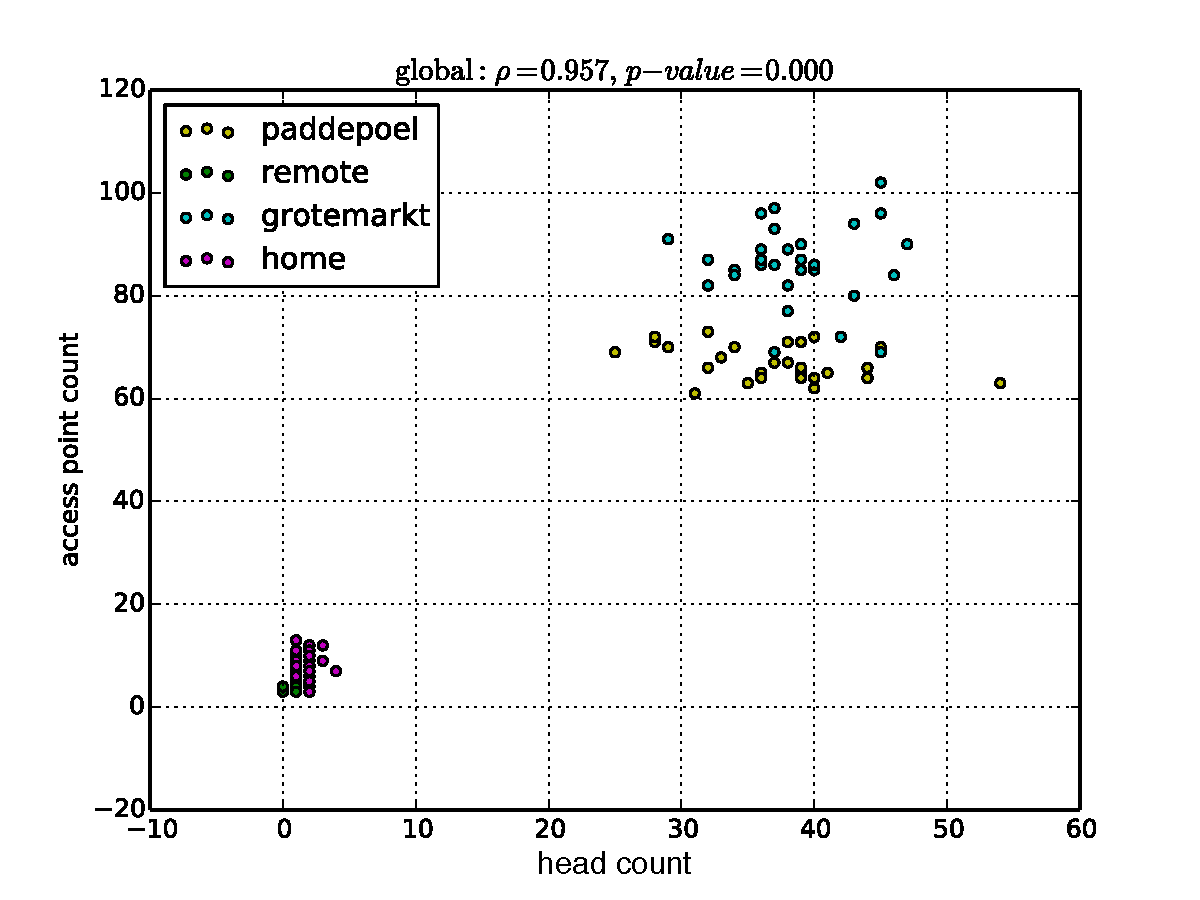
\includegraphics[width=0.7\textwidth]{./img/result/day/day1/global-gt-vs-ap}
    }
  }
  \subfloat[day 2]{
    \label{fig:ap-hc-day2}{
      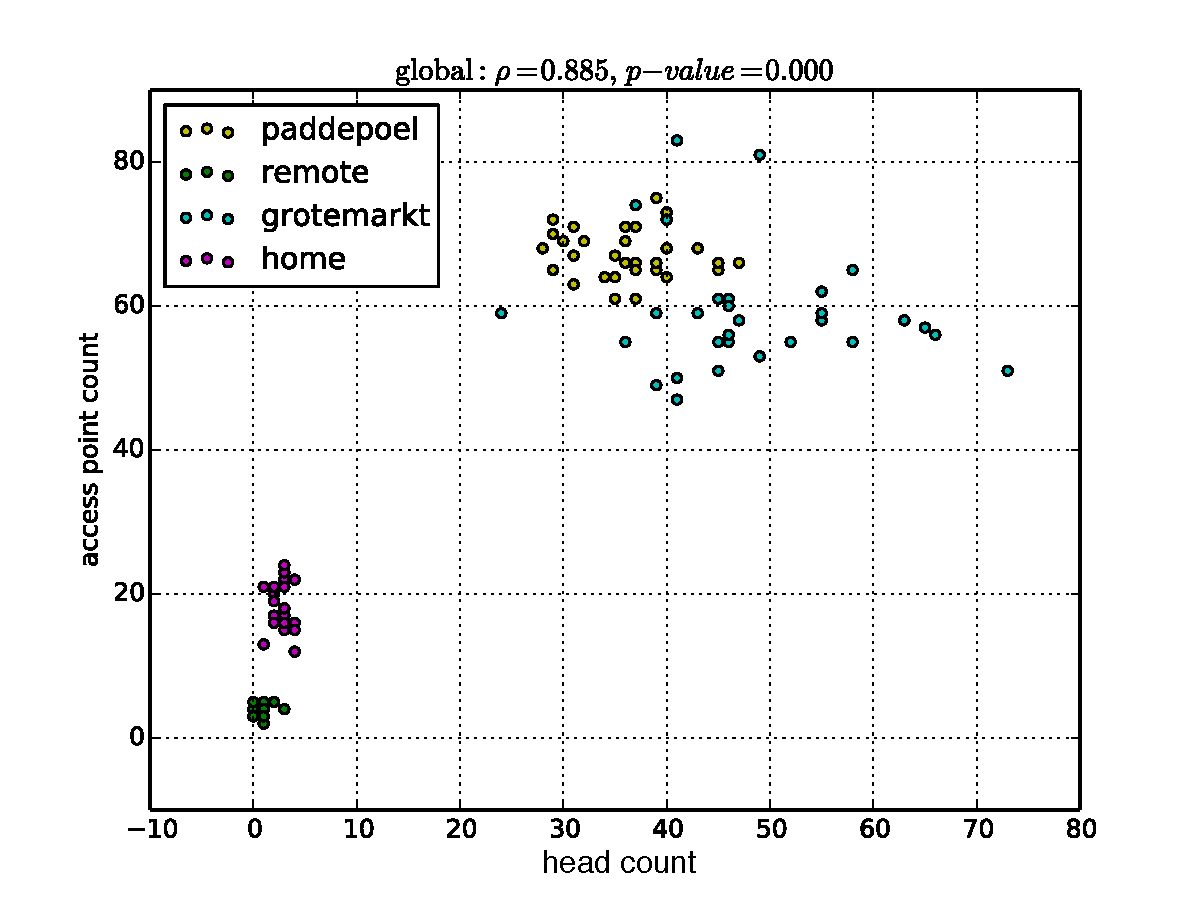
\includegraphics[width=0.7\textwidth]{./img/result/day/day2/global-gt-vs-ap}
    }
  }\\
  \subfloat[day 3]{
    \label{fig:ap-hc-day3}{
      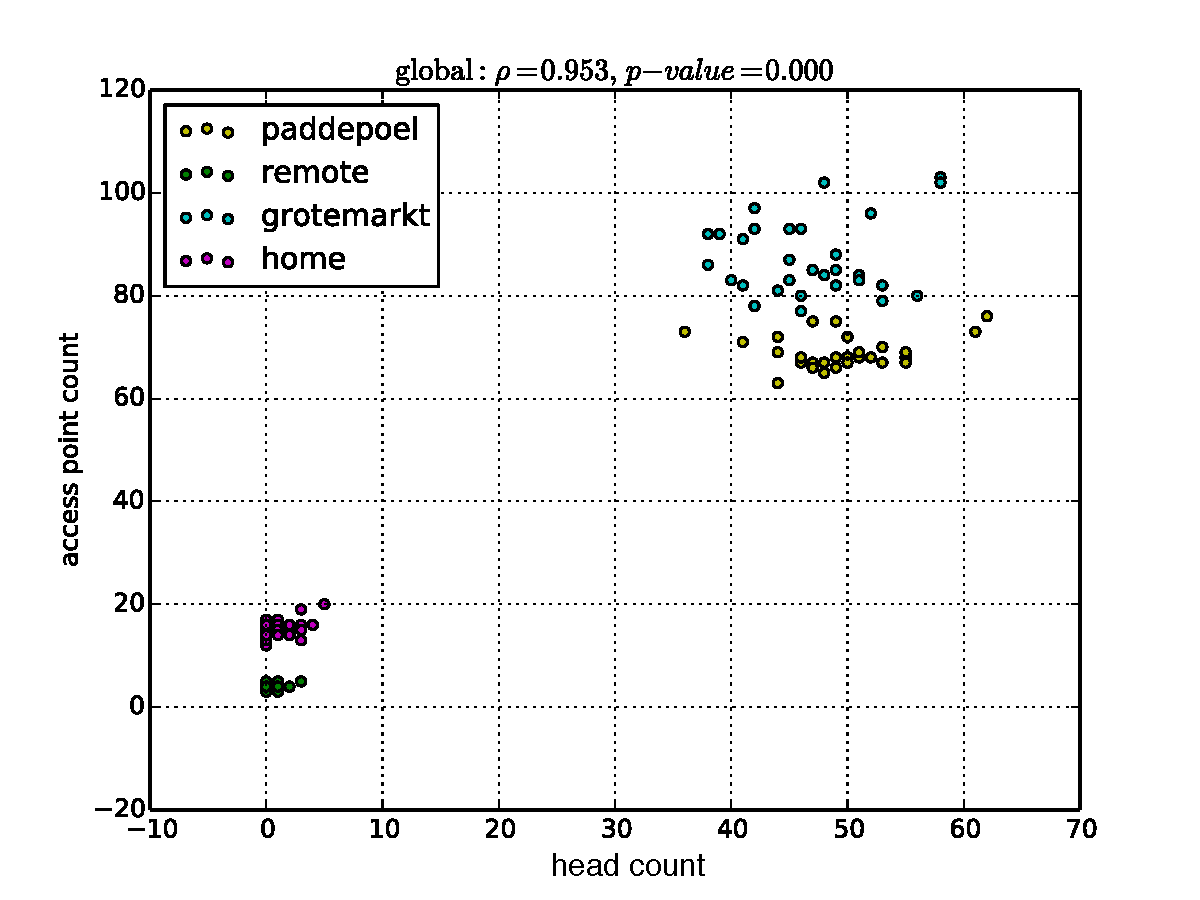
\includegraphics[width=0.7\textwidth]{./img/result/day/day3/global-gt-vs-ap}
    }
  }
  \subfloat[day 4]{
    \label{fig:ap-hc-day4}{
      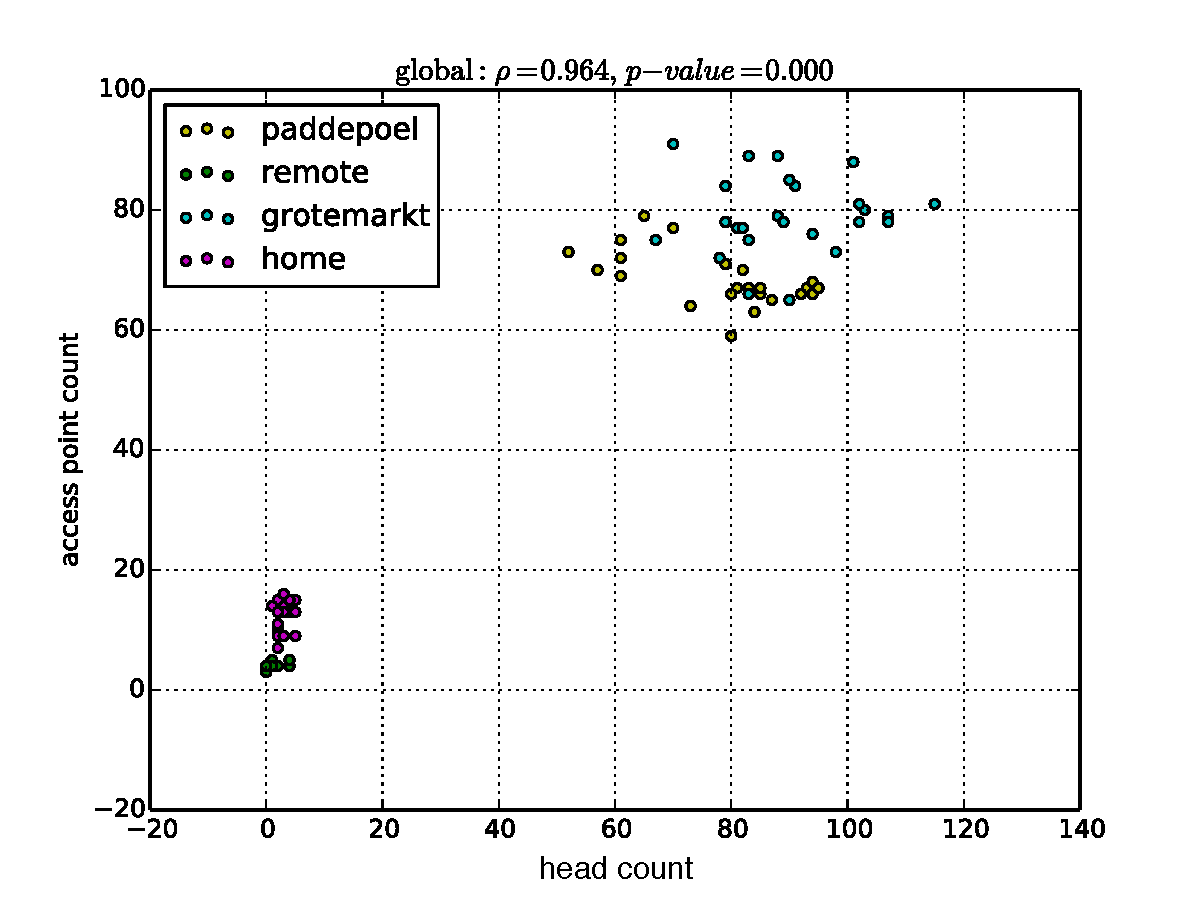
\includegraphics[width=0.7\textwidth]{./img/result/day/day4/global-gt-vs-ap}
    }
  }
  \end{adjustwidth}
  \caption[The scatter plots of the correlation between headcount and \ac{AP} count.]
  {The scatter plots showing the correlation between headcount and \ac{AP} count in four days of experiment. The location is coded in color.}
  \label{fig:ap-hc-scatterplot}
\end{figure}

% ap vs device count
\begin{figure}[H]
  \begin{adjustwidth}{-4cm}{}
  \centering
  \subfloat[day 1]{
    \label{fig:ap-dc-day1}{
      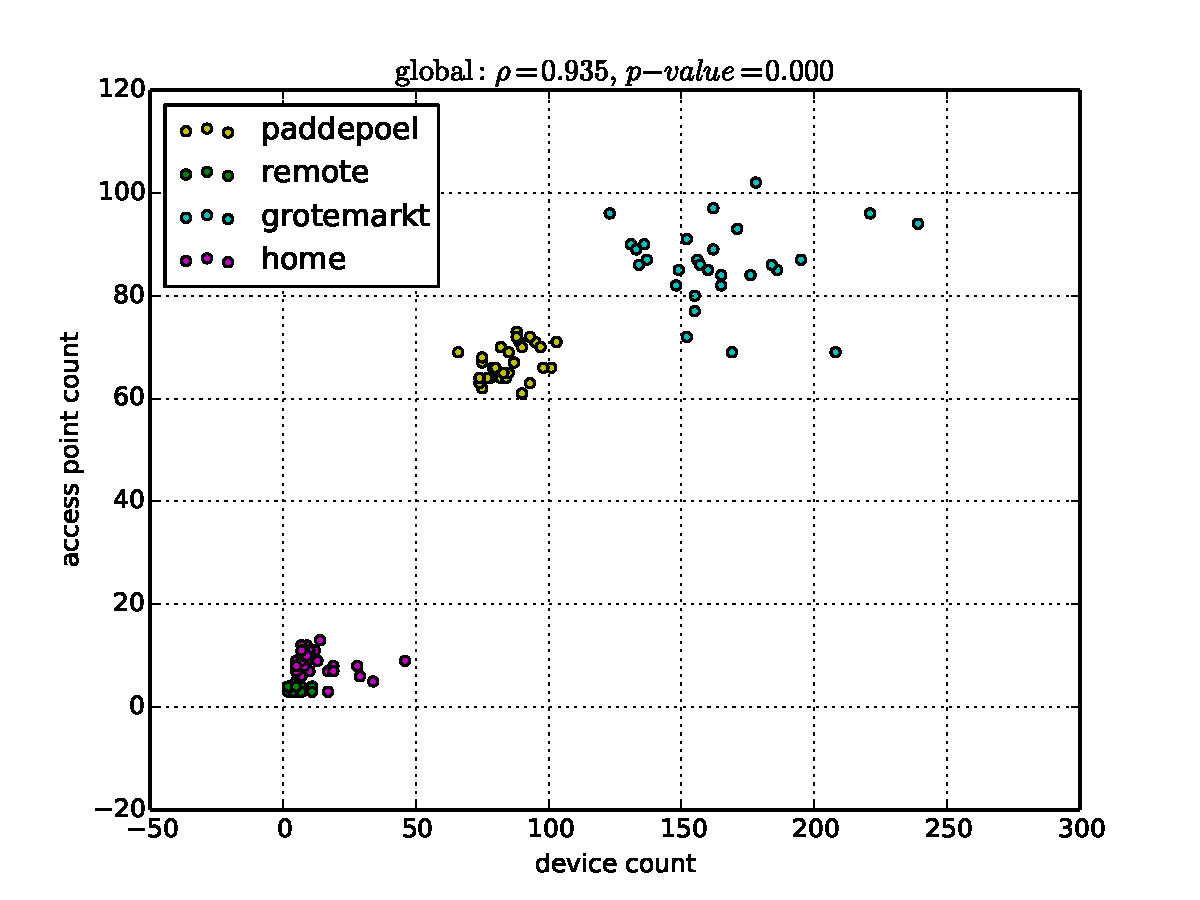
\includegraphics[width=0.7\textwidth]{./img/result/day/day1/global-pr-vs-ap}
    }
  }
  \subfloat[day 2]{
    \label{fig:ap-dc-day2}{
      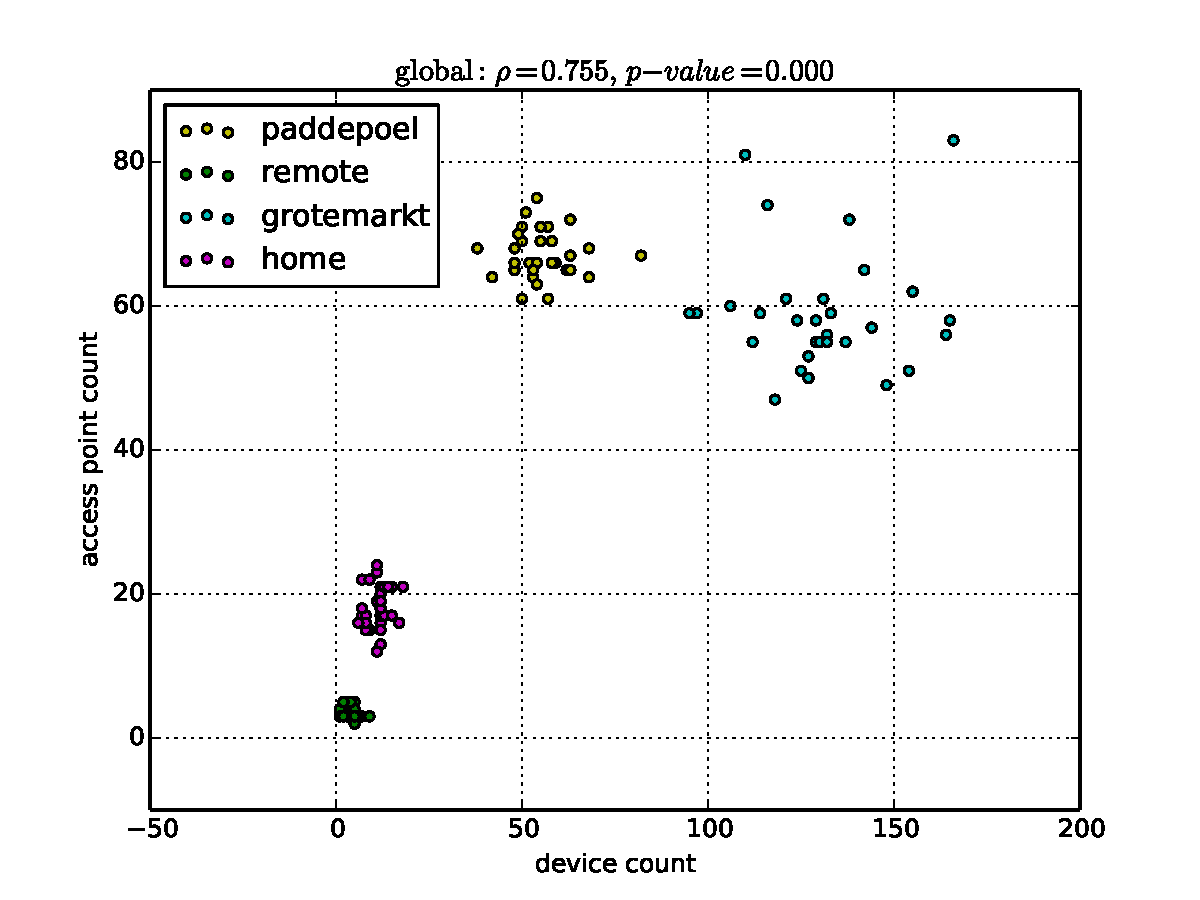
\includegraphics[width=0.7\textwidth]{./img/result/day/day2/global-pr-vs-ap}
    }
  }\\
  \subfloat[day 3]{
    \label{fig:ap-dc-day3}{
      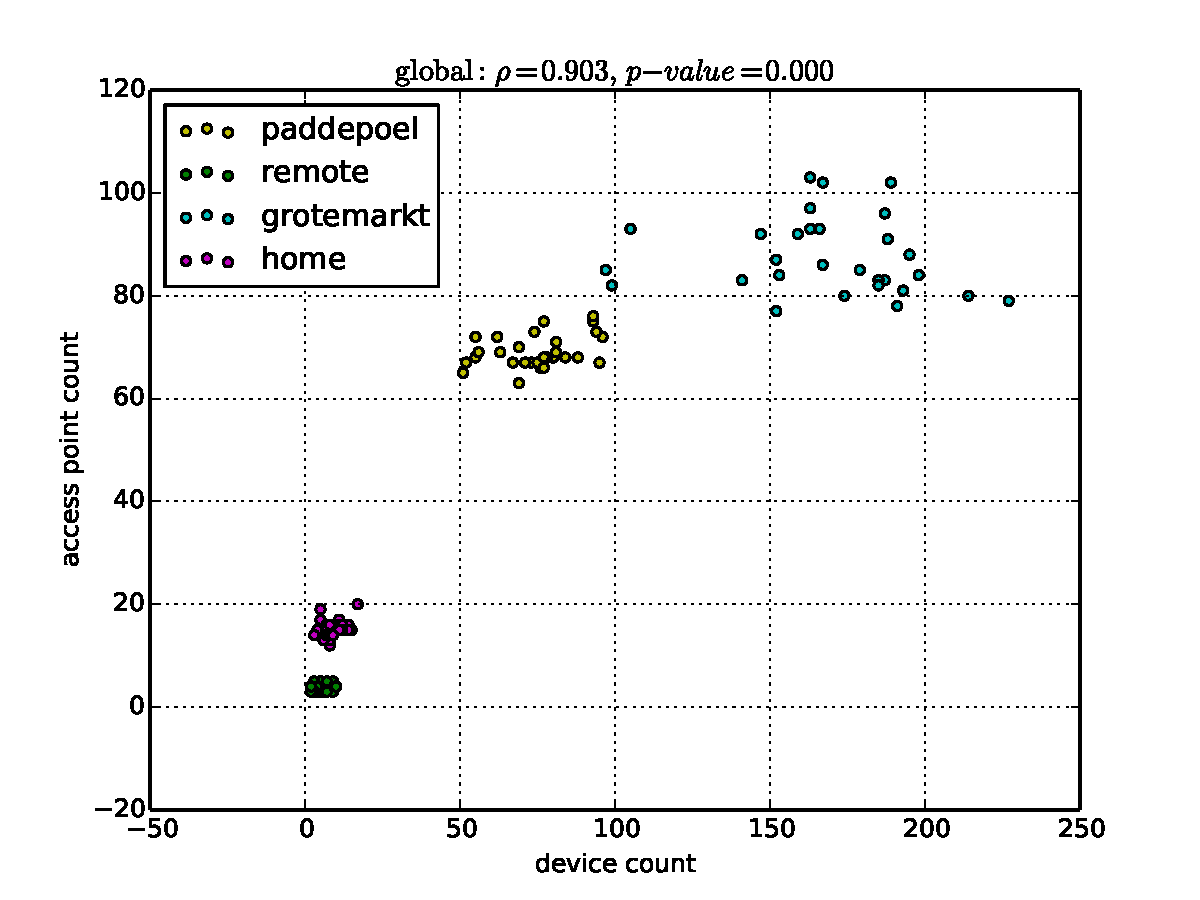
\includegraphics[width=0.7\textwidth]{./img/result/day/day3/global-pr-vs-ap}
    }
  }
  \subfloat[day 4]{
    \label{fig:ap-dc-day4}{
      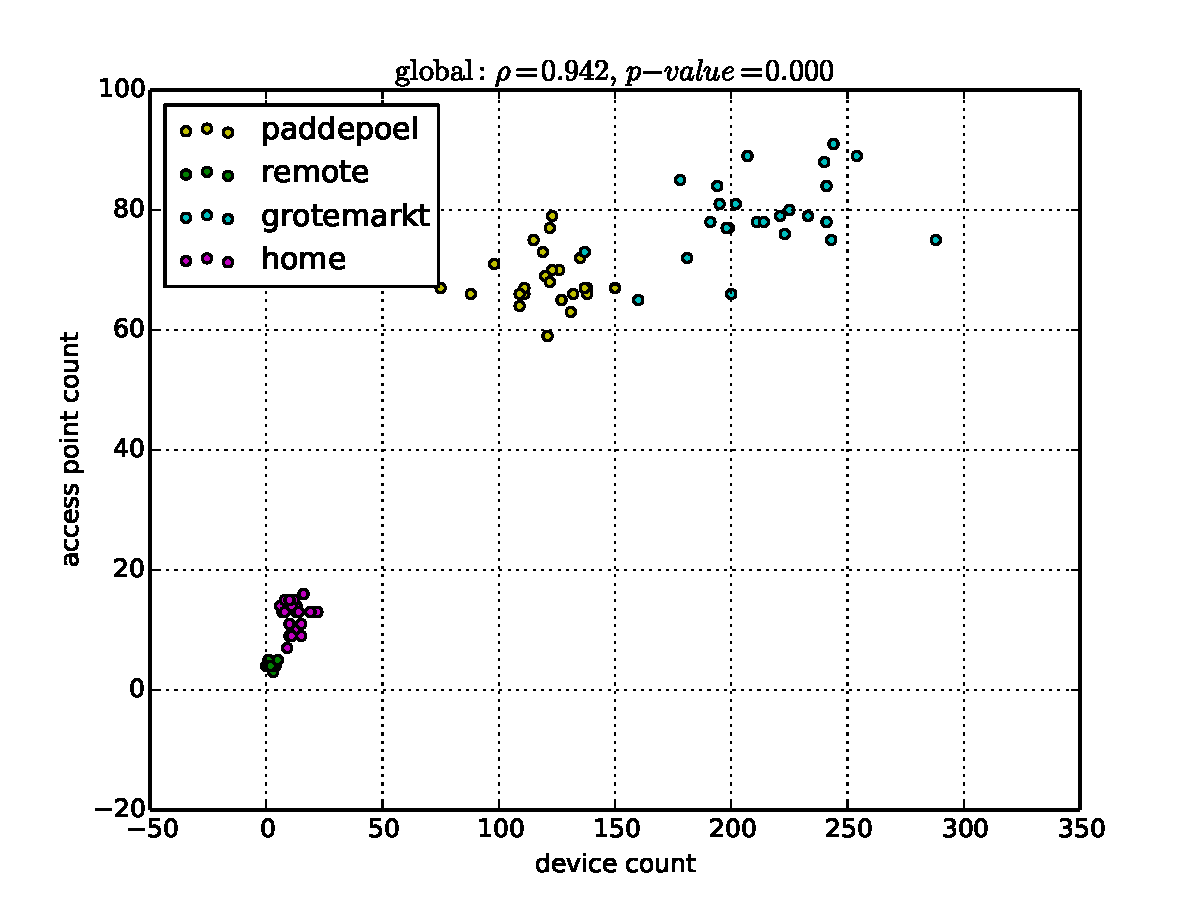
\includegraphics[width=0.7\textwidth]{./img/result/day/day4/global-pr-vs-ap}
    }
  }
  \end{adjustwidth}
  \caption[The scatter plots of the correlation between device count and \ac{AP}.]
  {The scatter plots showing the correlation between device count and \ac{AP} count in four days of experiment. The location is coded in color.}
  \label{fig:ap-dc-scatterplot}
\end{figure}

% ap vs device count
\begin{figure}[H]
  \begin{adjustwidth}{-1cm}{}
  \centering
  \subfloat[day 1]{
    \label{fig:hc-dc-day1}{
      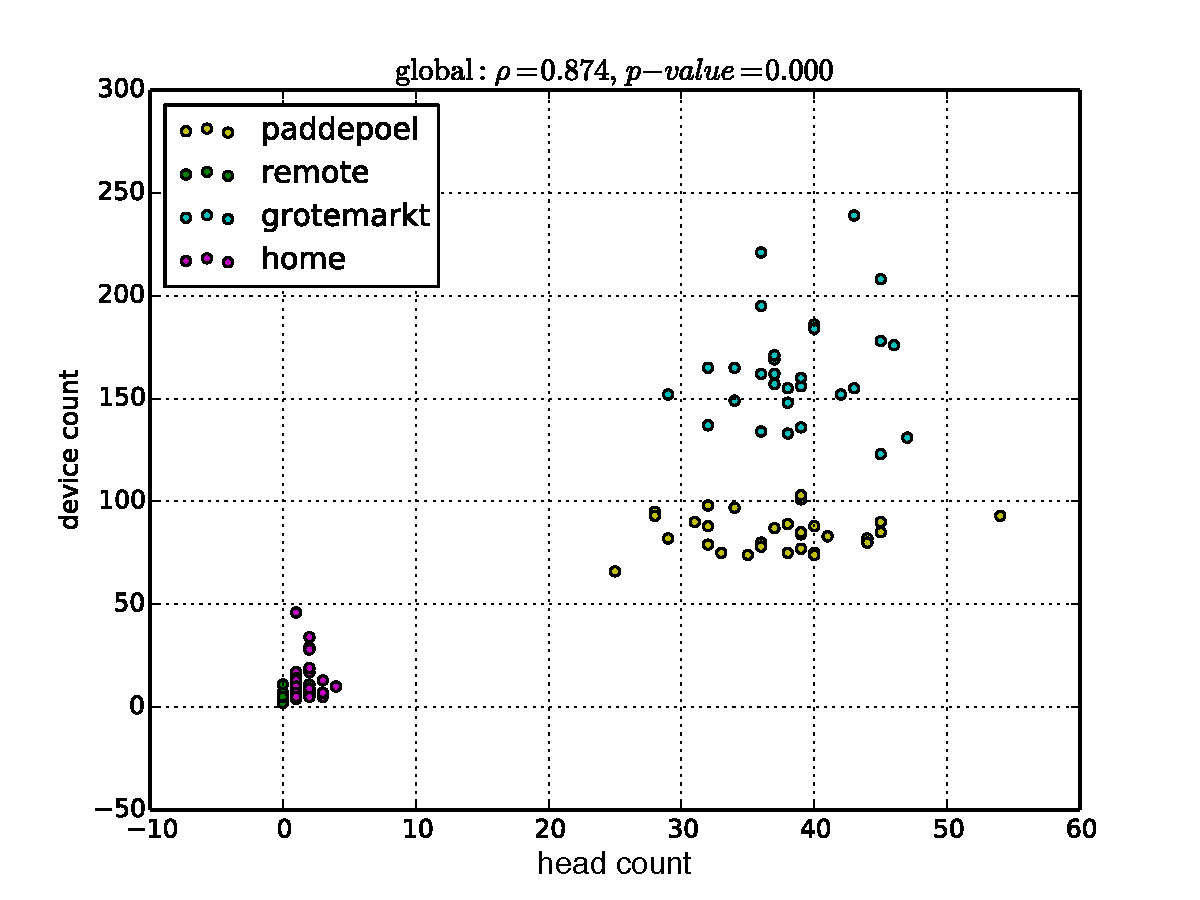
\includegraphics[width=0.7\textwidth]{./img/result/day/day1/global-gt-vs-pr}
    }
  }
  \subfloat[day 2]{
    \label{fig:hc-dc-day2}{
      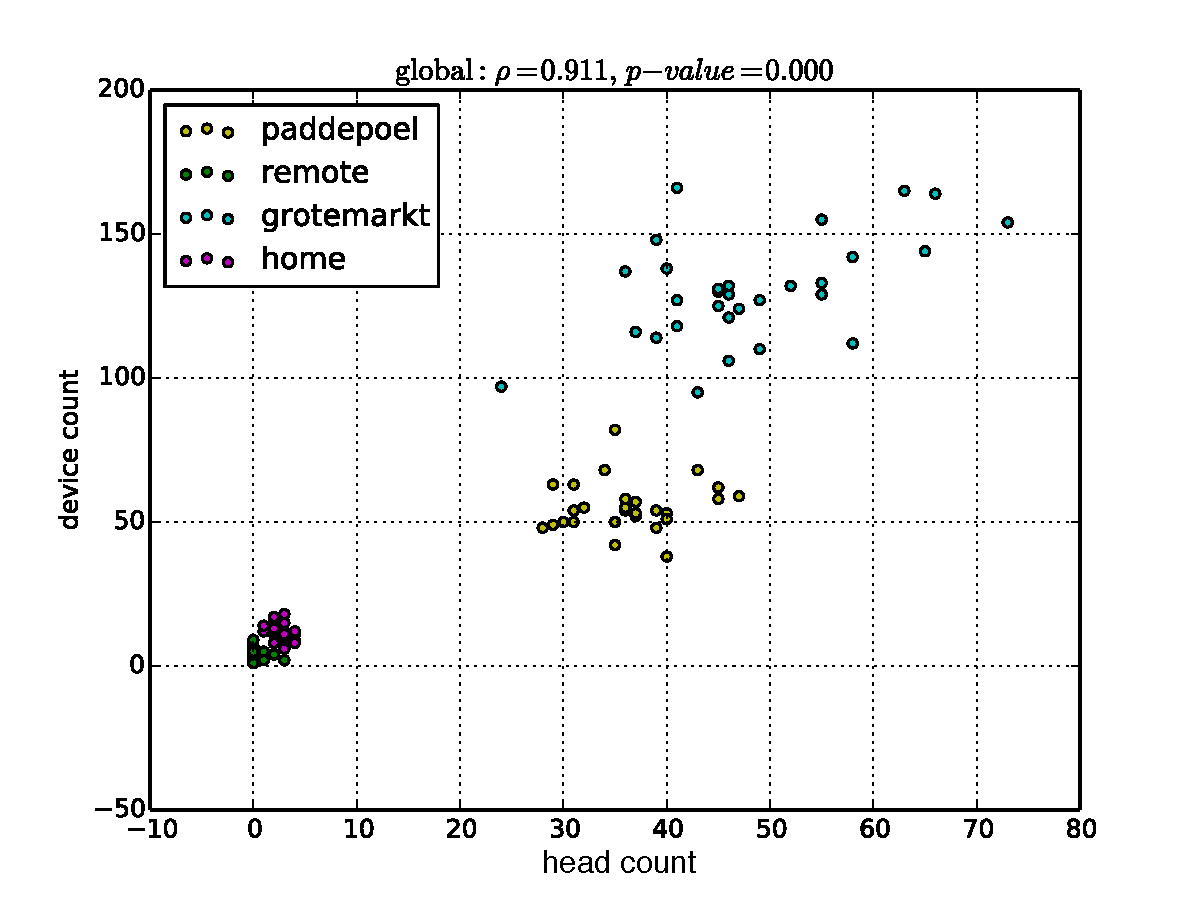
\includegraphics[width=0.7\textwidth]{./img/result/day/day2/global-gt-vs-pr}
    }
  }\\
  \subfloat[day 3]{
    \label{fig:hc-dc-day3}{
      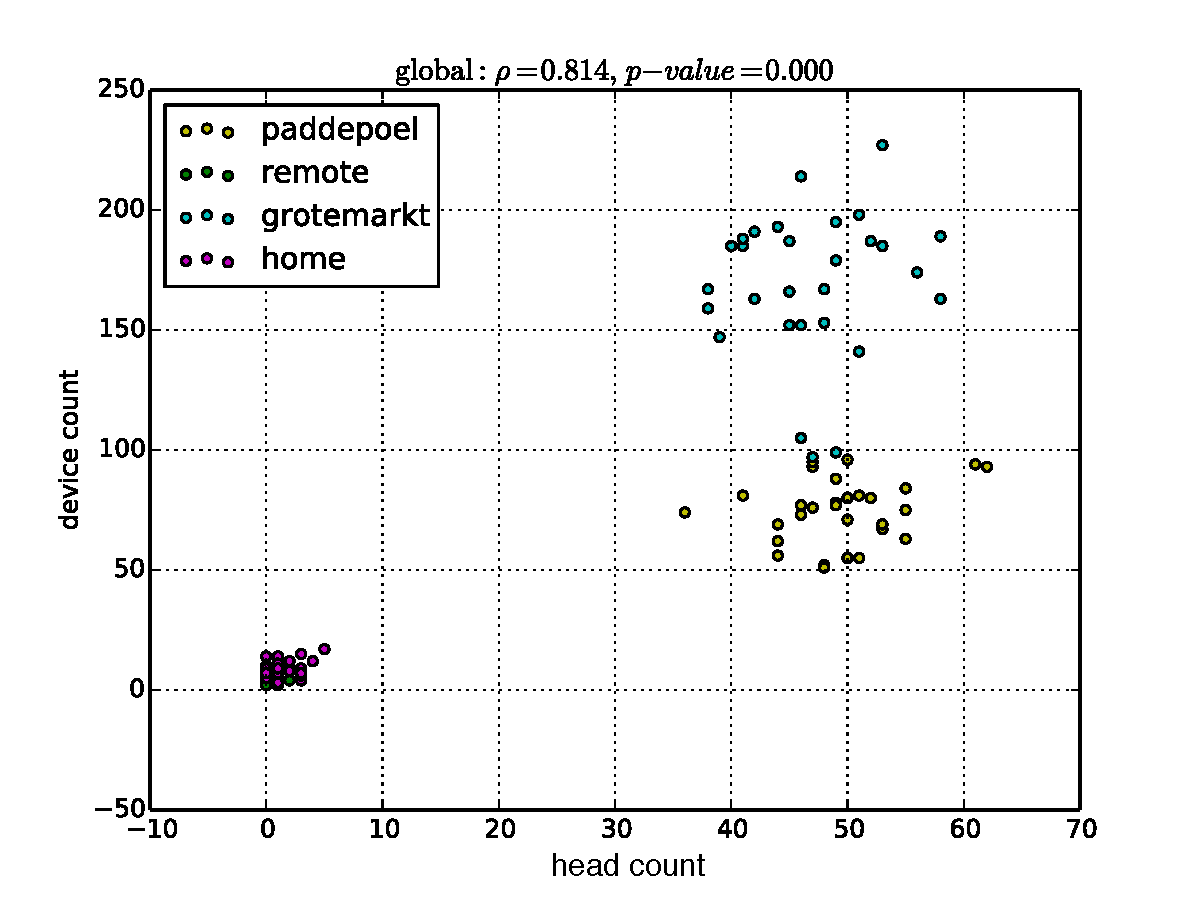
\includegraphics[width=0.7\textwidth]{./img/result/day/day3/global-gt-vs-pr}
    }
  }
  \subfloat[day 4]{
    \label{fig:hc-dc-day4}{
      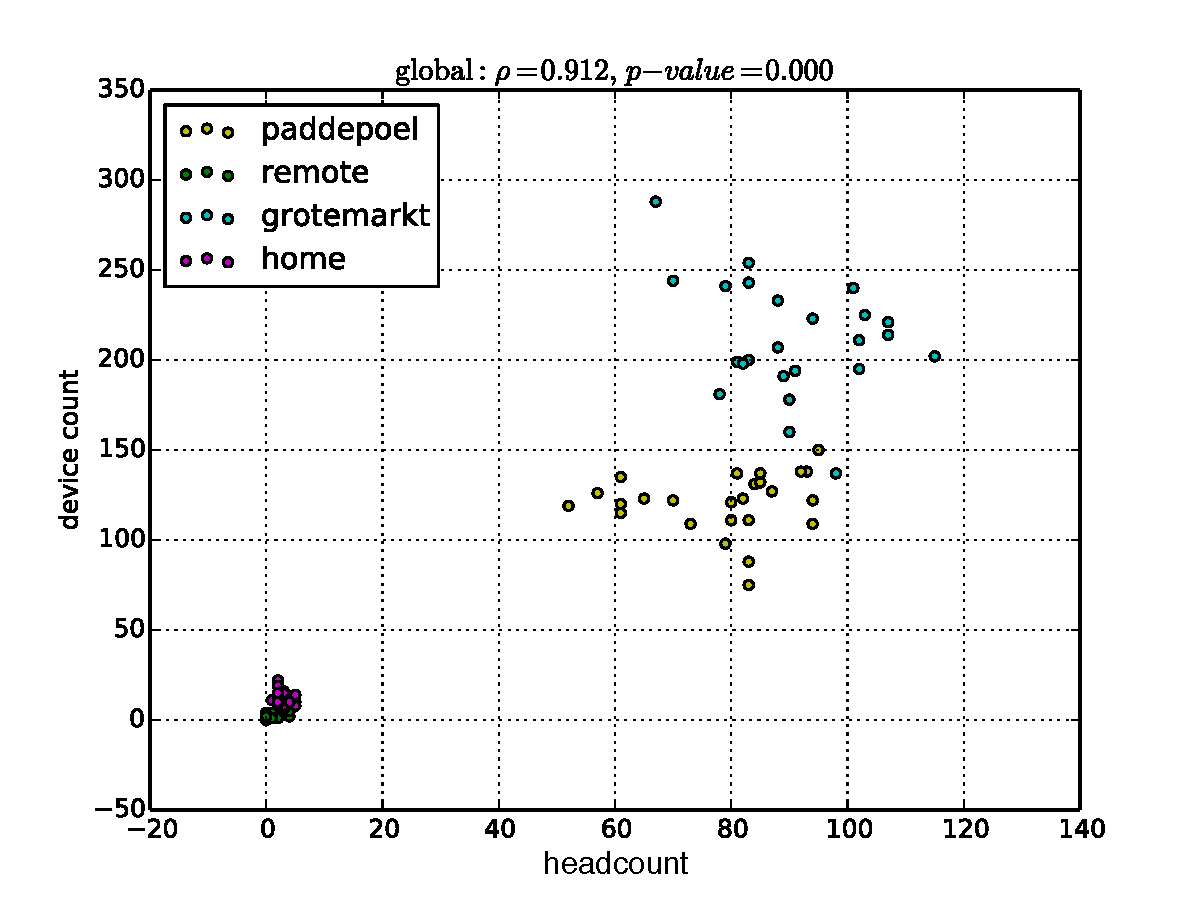
\includegraphics[width=0.7\textwidth]{./img/result/day/day4/global-gt-vs-pr}
    }
  }
  \end{adjustwidth}
  \caption[The scatter plots of the correlation between device count and \ac{AP} count.]
  {The scatter plots showing the correlation between device count and \ac{AP} count in four days of experiment. The location is coded in color.}
  \label{fig:hc-dc-scatterplot}
\end{figure}







\section{Line charts} % (fold)
\label{sec:line_charts}

\begin{figure}[H]
  \begin{adjustwidth}{-4.5cm}{}
  \centering
  \subfloat[day 1]{
    \label{fig:remote-day1}{
      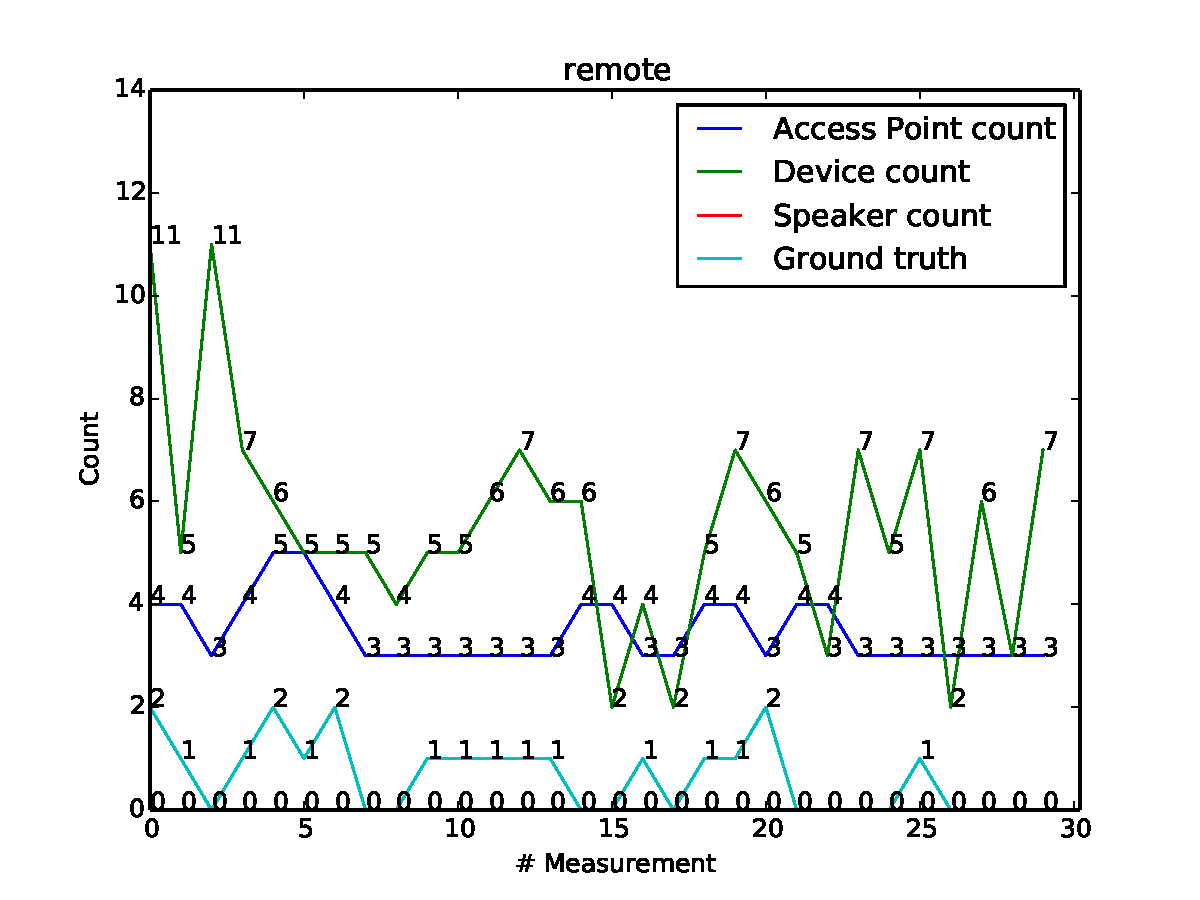
\includegraphics[width=0.7\textwidth]{./img/result/day/day1/remote-20161026}
    }
  }
  \subfloat[day 2]{
    \label{fig:remote-day2}{
      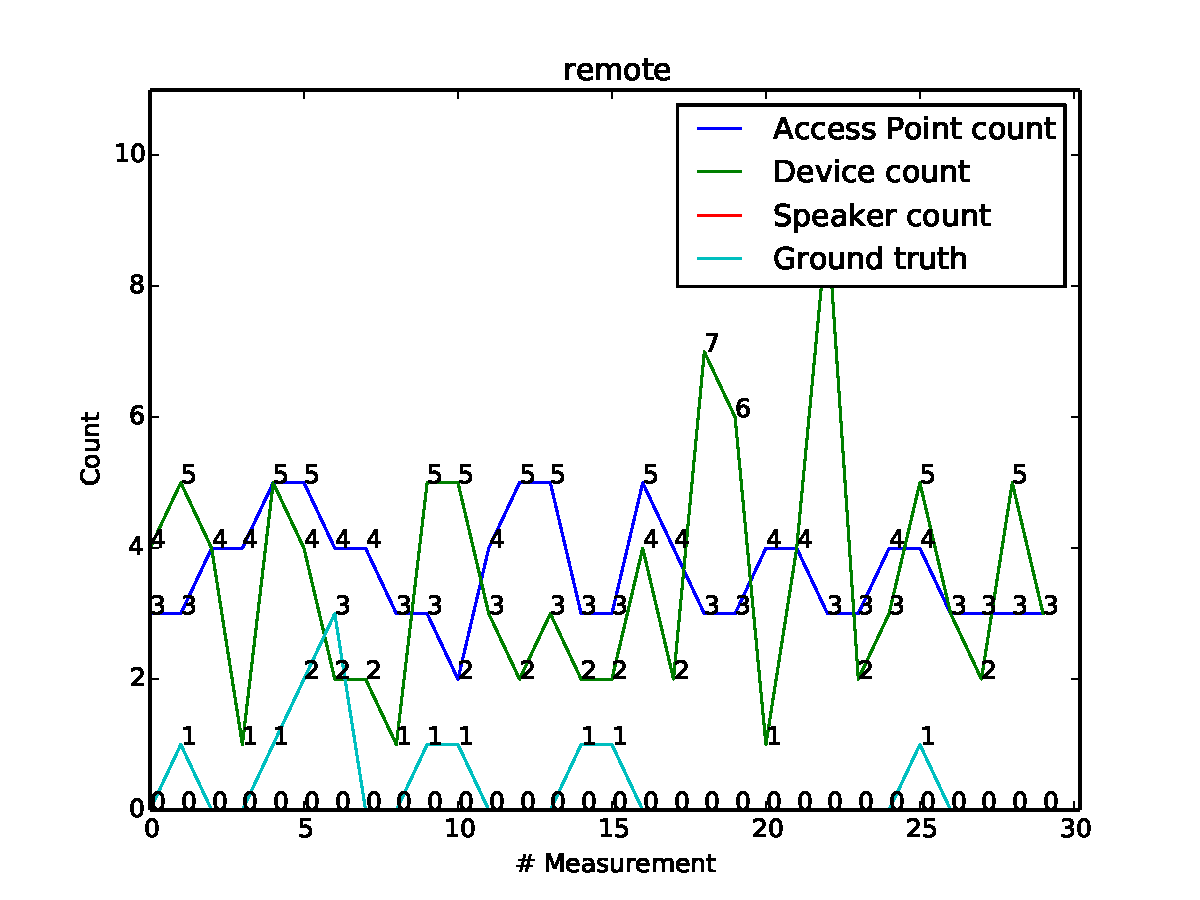
\includegraphics[width=0.7\textwidth]{./img/result/day/day2/remote-20161027}
    }
  }\\
  \subfloat[day 3]{
    \label{fig:remote-day3}{
      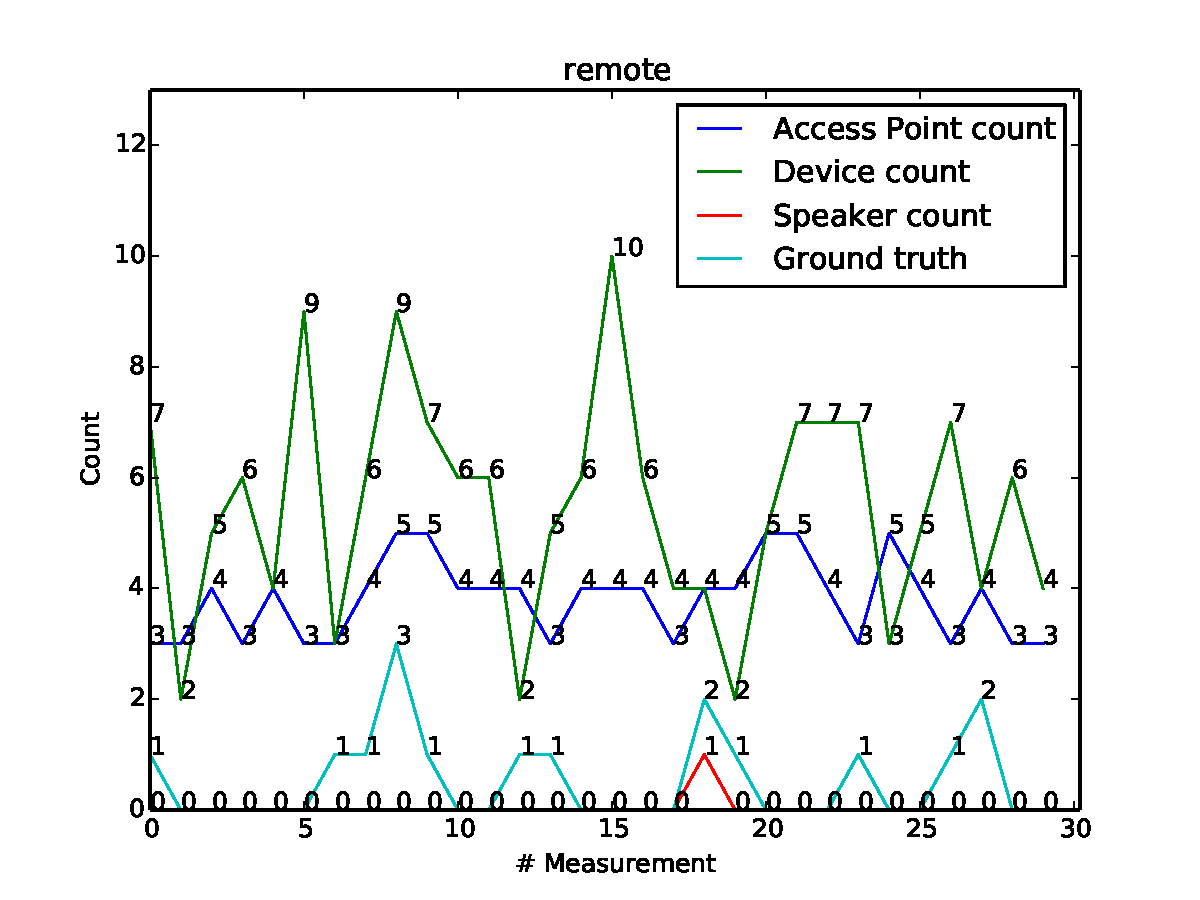
\includegraphics[width=0.7\textwidth]{./img/result/day/day3/remote-20161028}
    }
  }
  \subfloat[day 4]{
    \label{fig:remote-day4}{
      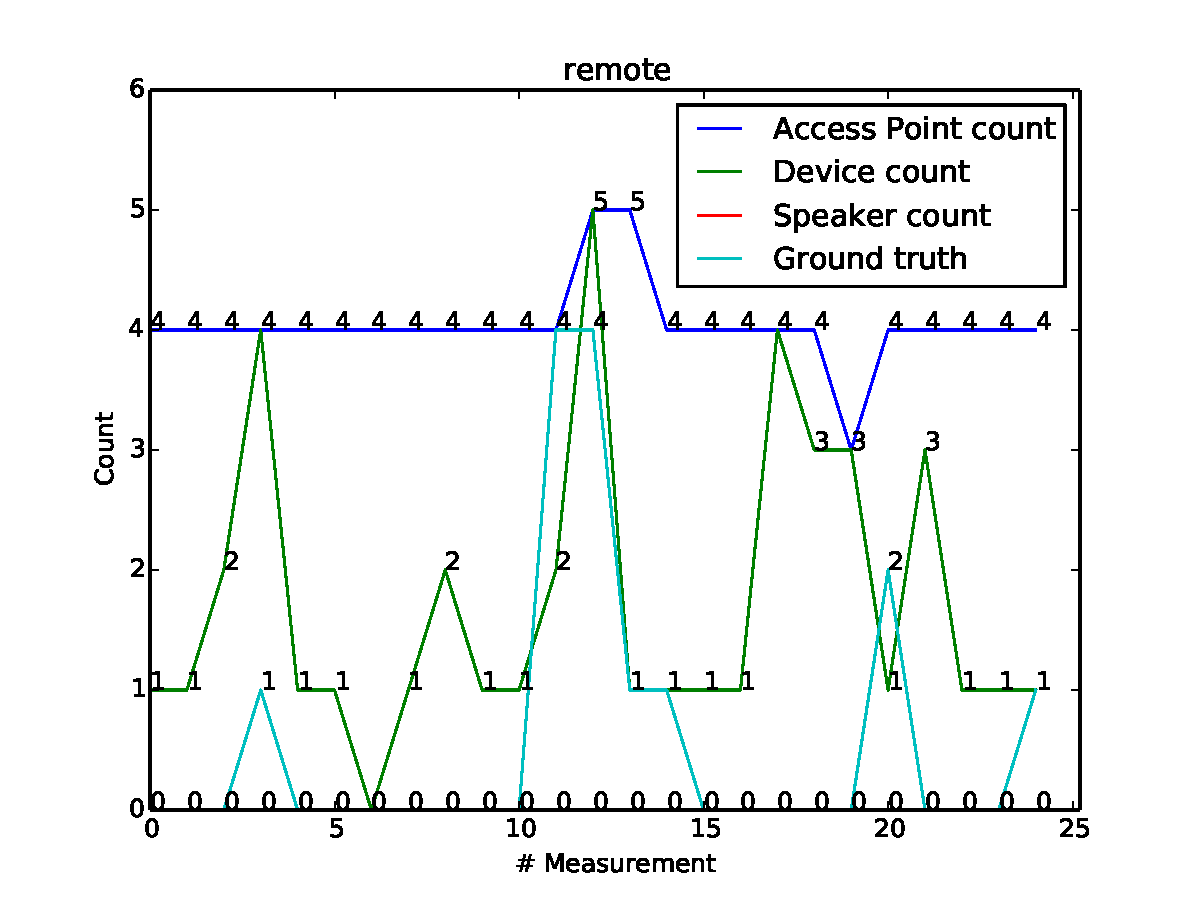
\includegraphics[width=0.7\textwidth]{./img/result/day/day4/remote-20161029}
    }
  }
  \end{adjustwidth}
  \caption[The line chart of sensor readings at remote area.]
  {The line chart of sensor readings at \textit{remote area} in four days of experiment.}
  \label{fig:result-remote-line-chart}
\end{figure}


\begin{figure}[H]
  \begin{adjustwidth}{-1cm}{}
  \centering
  \subfloat[day 1]{
    \label{fig:home-day1}{
      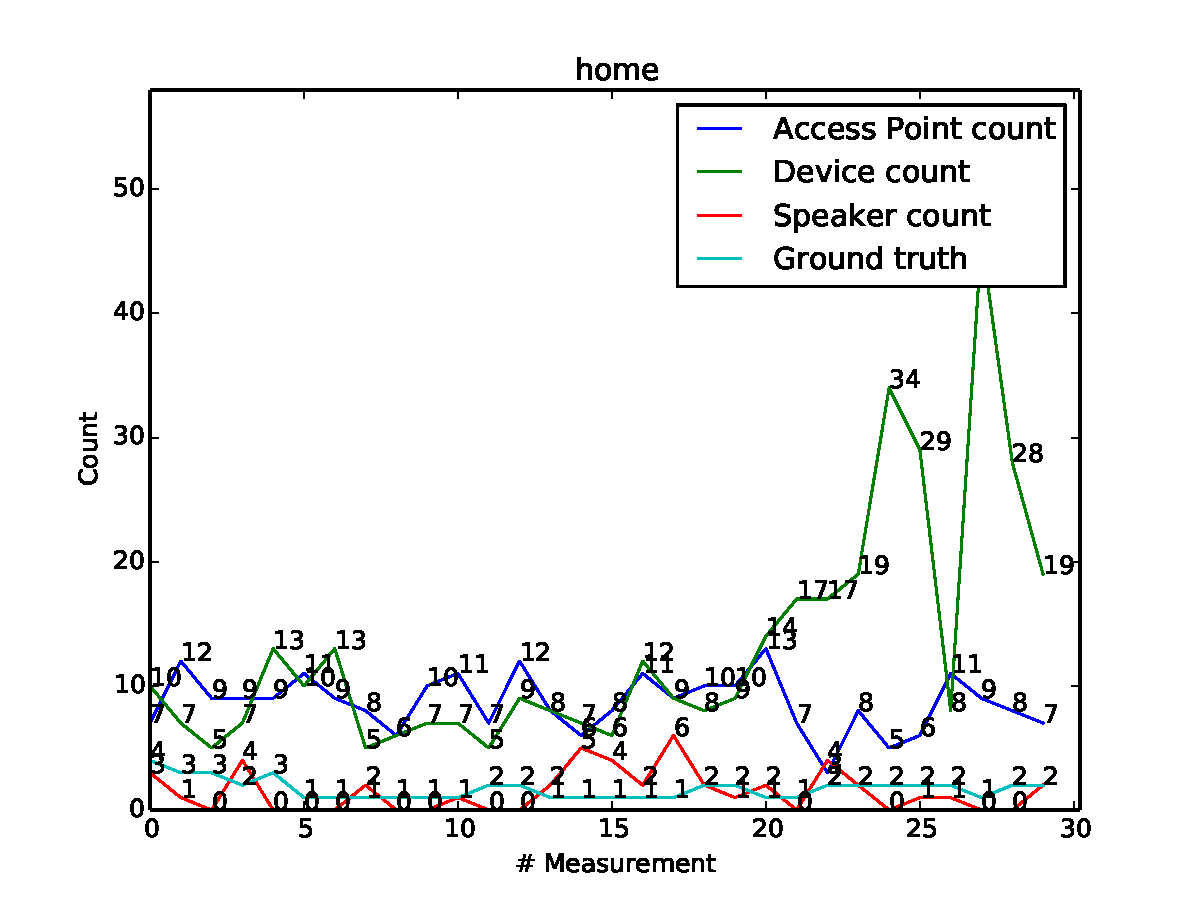
\includegraphics[width=0.7\textwidth]{./img/result/day/day1/home-20161026}
    }
  }
  \subfloat[day 2]{
    \label{fig:home-day2}{
      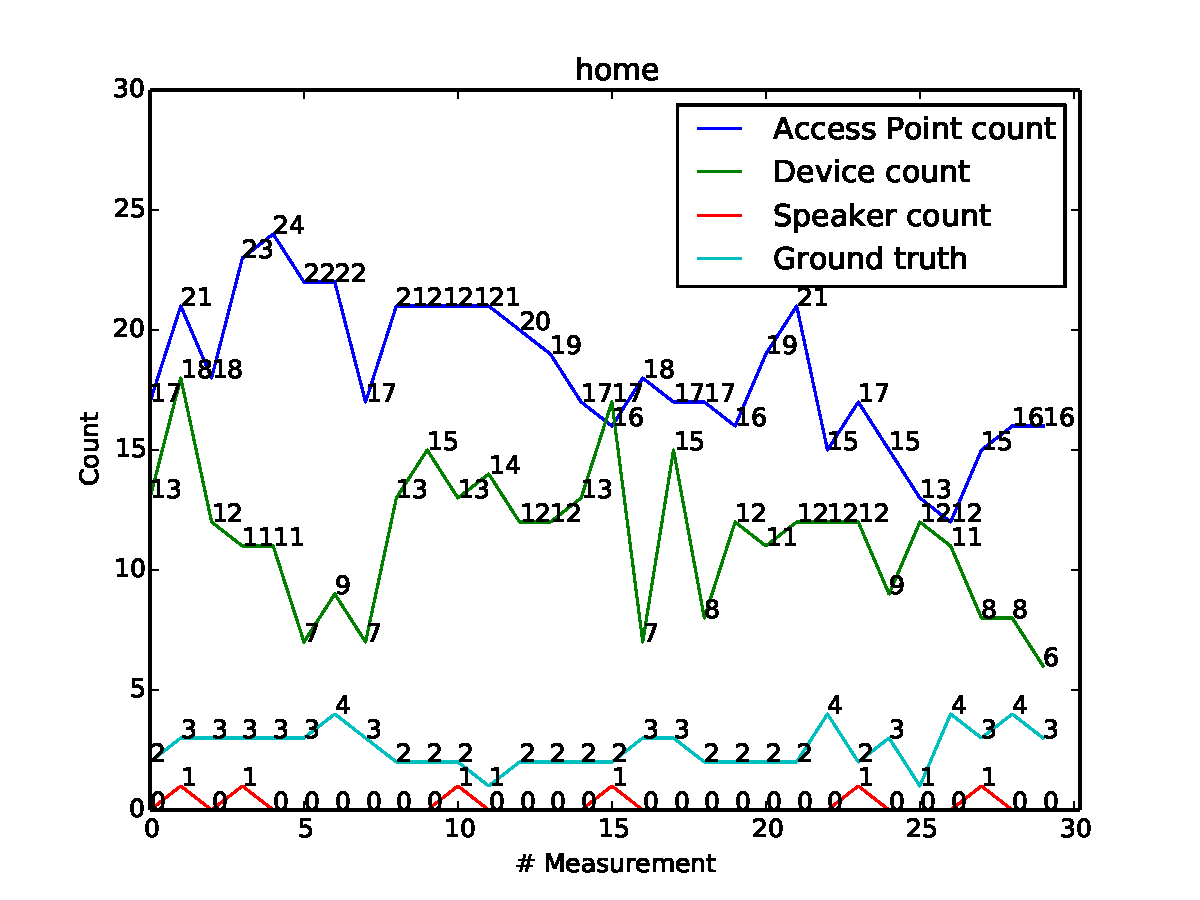
\includegraphics[width=0.7\textwidth]{./img/result/day/day2/home-20161027}
    }
  }\\
  \subfloat[day 3]{
    \label{fig:home-day3}{
      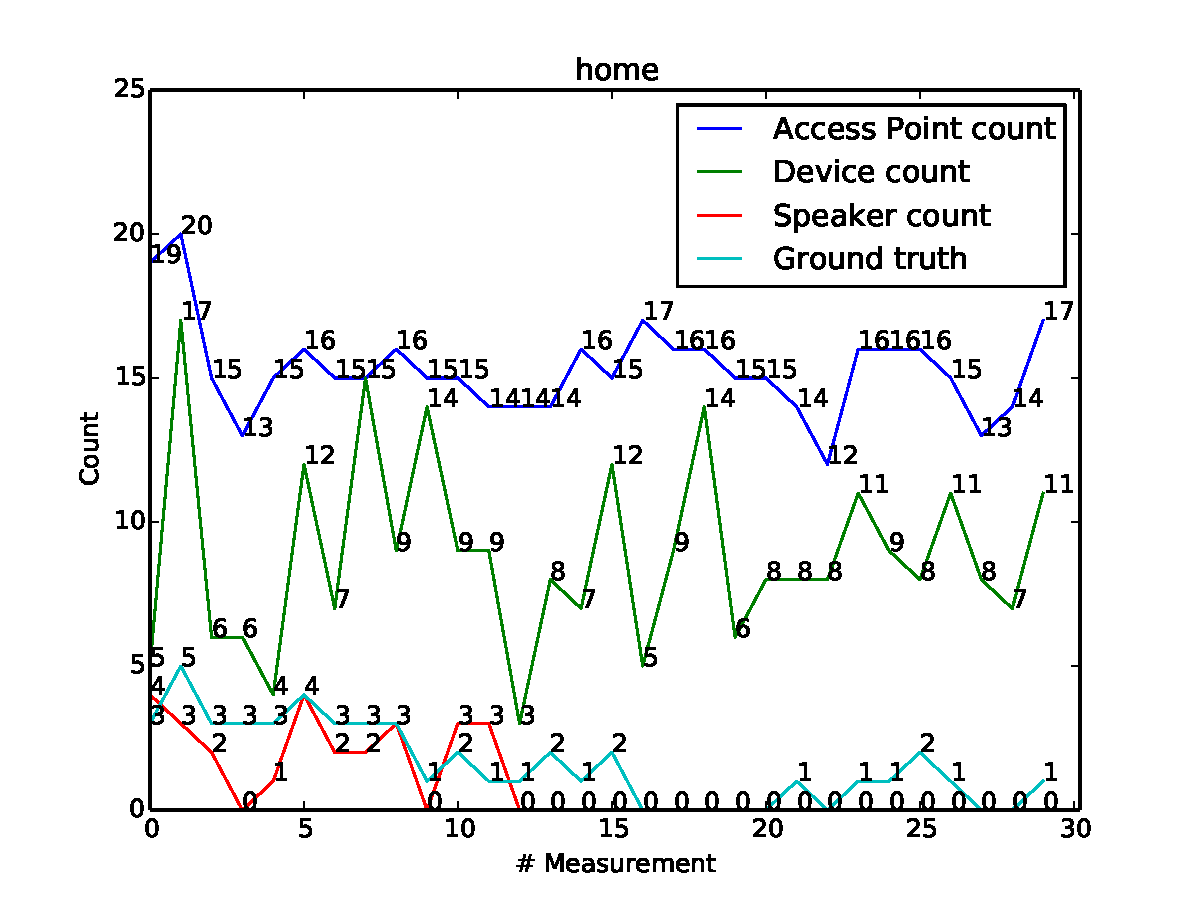
\includegraphics[width=0.7\textwidth]{./img/result/day/day3/home-20161028}
    }
  }
  \subfloat[day 4]{
    \label{fig:home-day4}{
      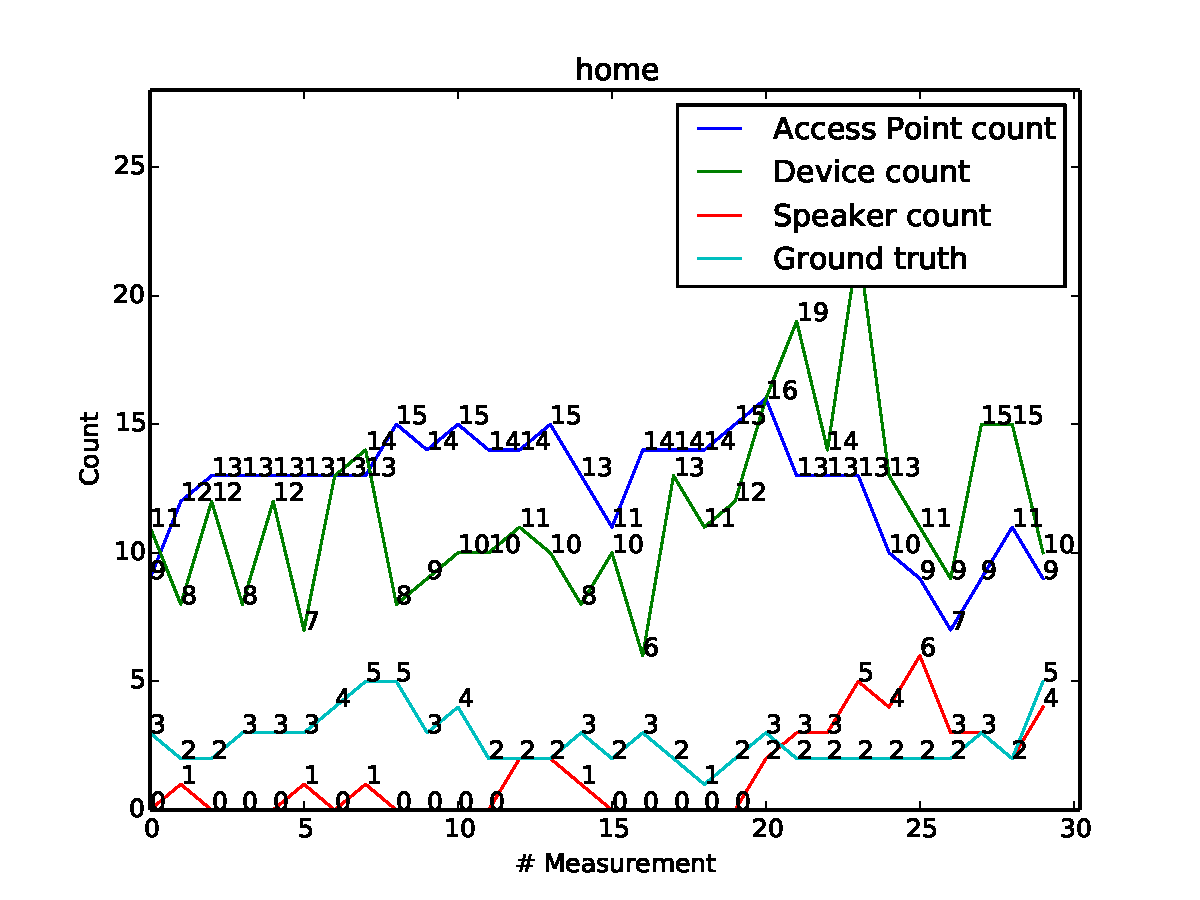
\includegraphics[width=0.7\textwidth]{./img/result/day/day4/home-20161029}
    }
  }
  \end{adjustwidth}
  \caption[The line chart of sensor readings at home.]
  {The line chart of sensor readings at \textit{home} in four days of experiment.}
  \label{fig:result-home-line-chart}
\end{figure}


\begin{figure}[H]
  \begin{adjustwidth}{-5cm}{}
  \centering
  \subfloat[day 1]{
    \label{fig:paddepoel-day1}{
      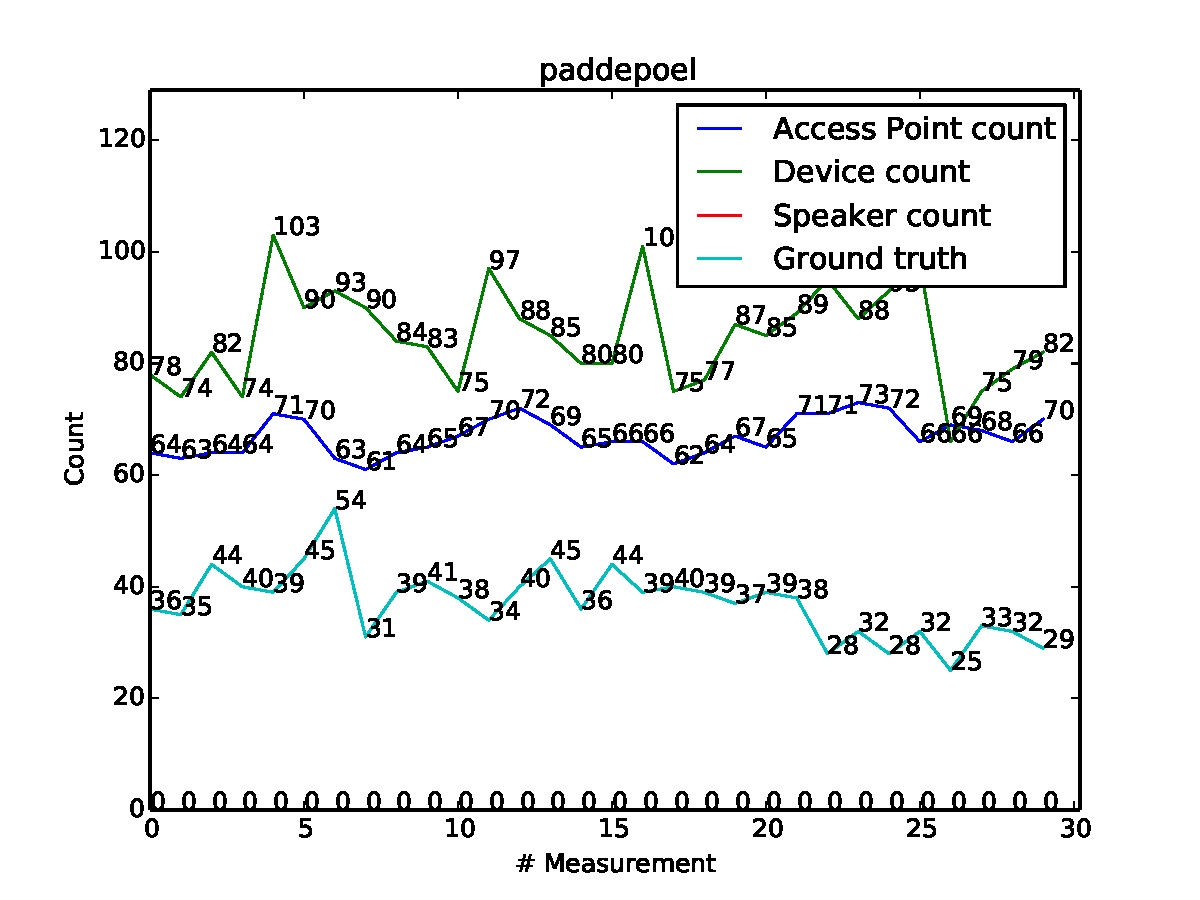
\includegraphics[width=0.7\textwidth]{./img/result/day/day1/paddepoel-20161026}
    }
  }
  \subfloat[day 2]{
    \label{fig:paddepoel-day2}{
      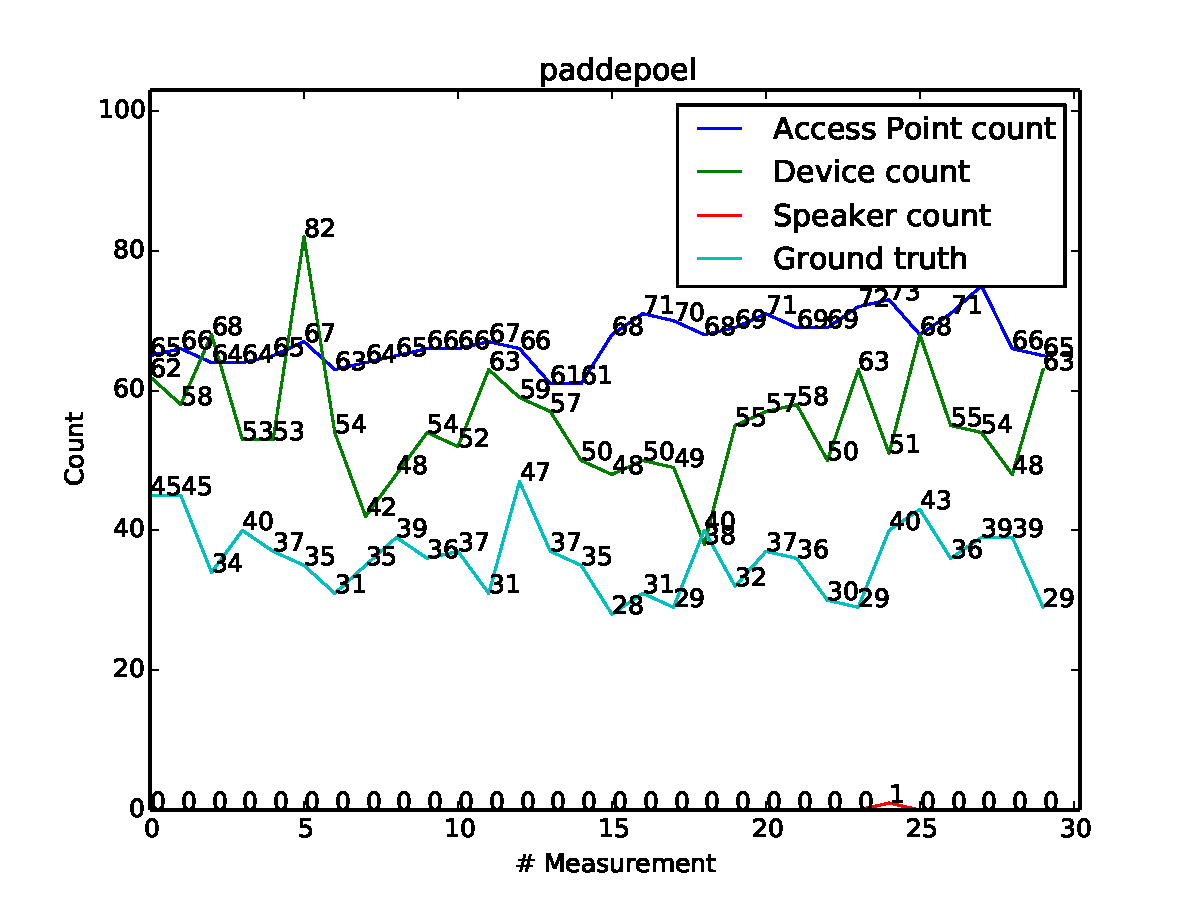
\includegraphics[width=0.7\textwidth]{./img/result/day/day2/paddepoel-20161027}
    }
  }\\
  \subfloat[day 3]{
    \label{fig:paddepoel-day3}{
      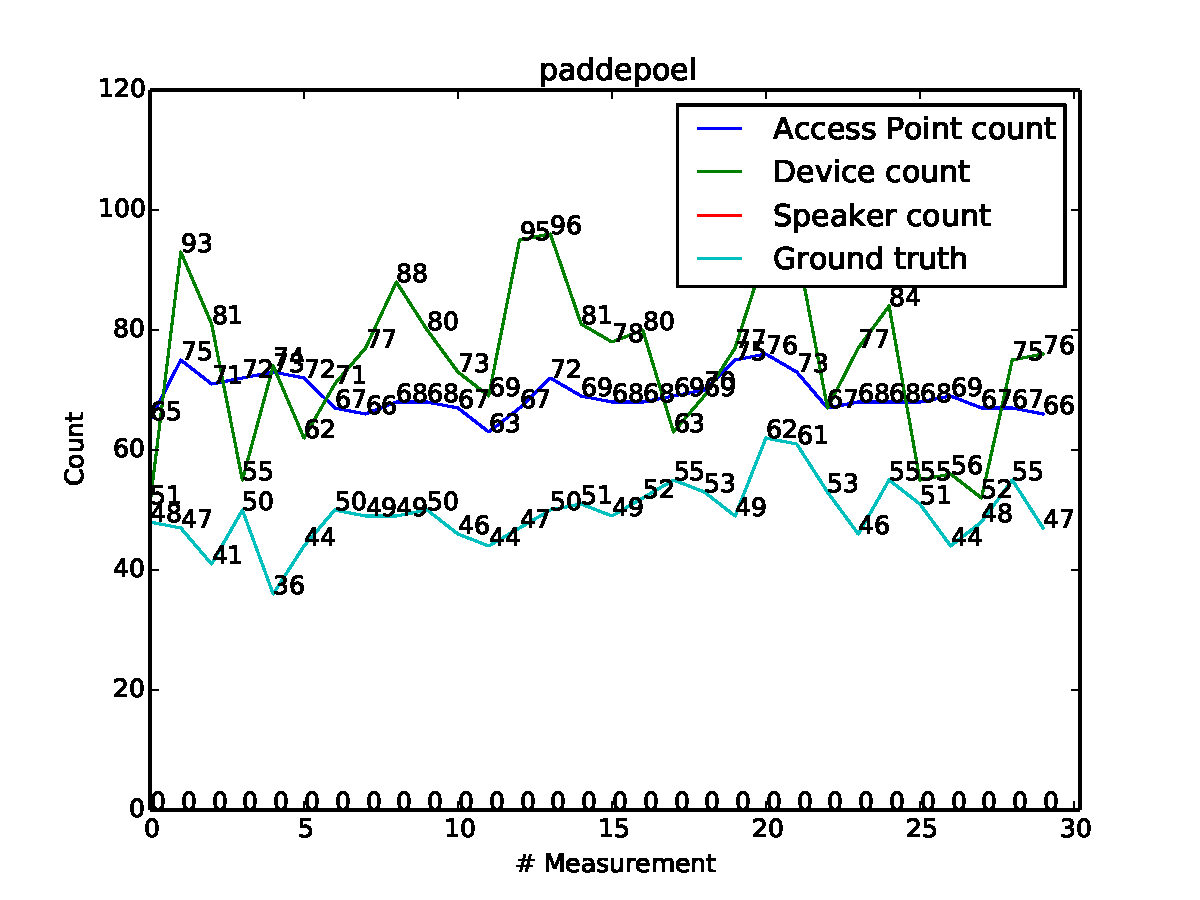
\includegraphics[width=0.7\textwidth]{./img/result/day/day3/paddepoel-20161028}
    }
  }
  \subfloat[day 4]{
    \label{fig:paddepoel-day4}{
      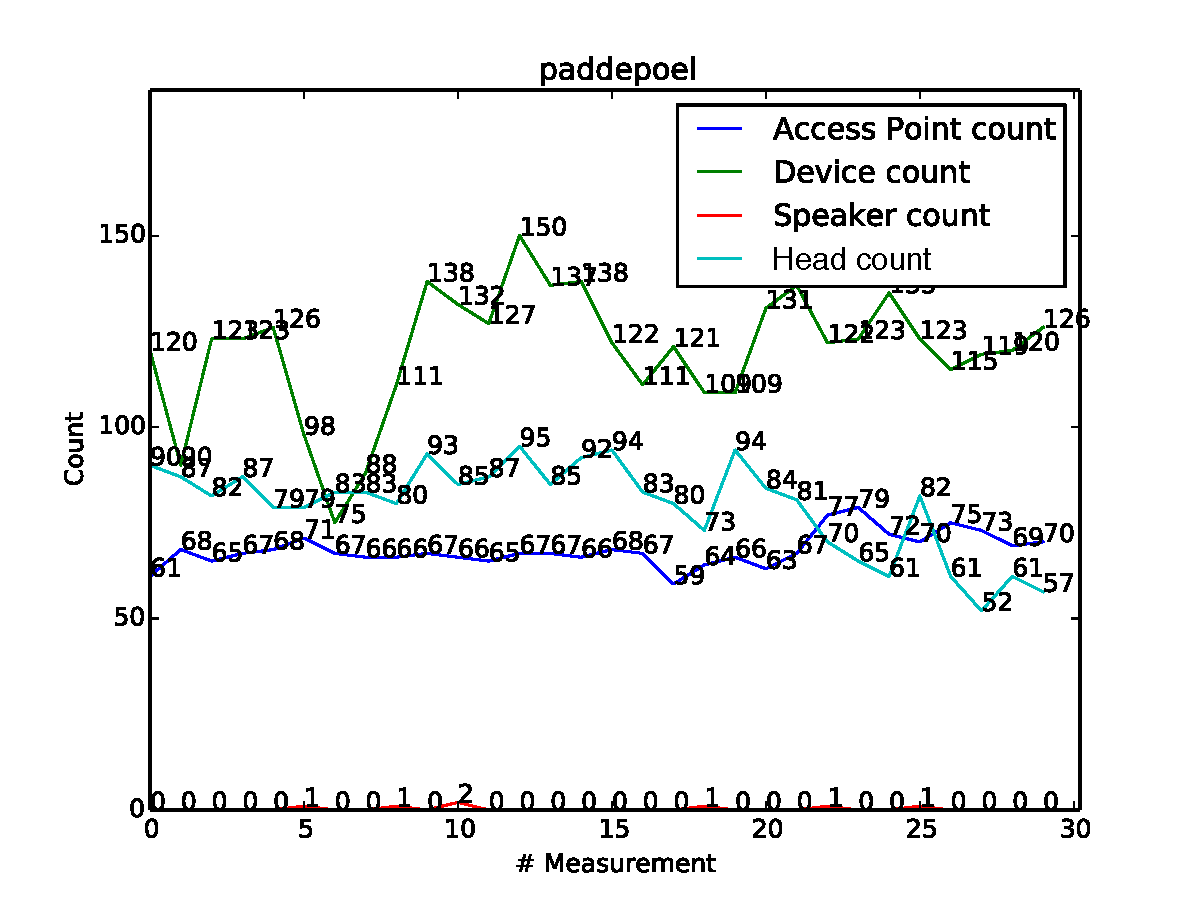
\includegraphics[width=0.7\textwidth]{./img/result/day/day4/paddepoel-20161029}
    }
  }
  \end{adjustwidth}
  \caption[The line chart of sensor readings at Paddepoel Shopping Center.]
  {The line chart of sensor readings at \textit{Paddepoel Shopping Center} in four days of experiment.}
  \label{fig:result-paddepoel-line-chart}
\end{figure}


\begin{figure}[H]
  \begin{adjustwidth}{-1cm}{}
  \centering
  \subfloat[day 1]{
    \label{fig:grotemarkt-day1}{
      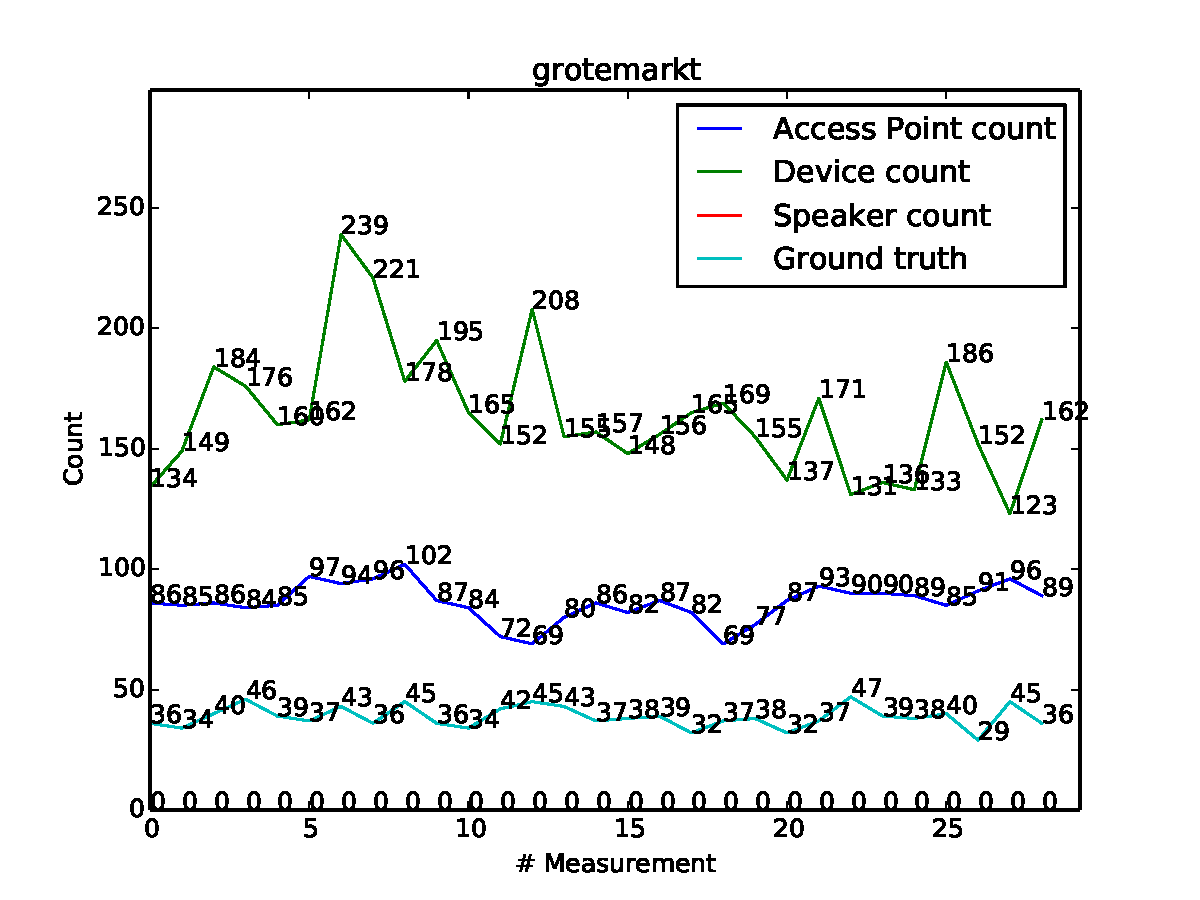
\includegraphics[width=0.7\textwidth]{./img/result/day/day1/grotemarkt-20161026}
    }
  }
  \subfloat[day 2]{
    \label{fig:grotemarkt-day2}{
      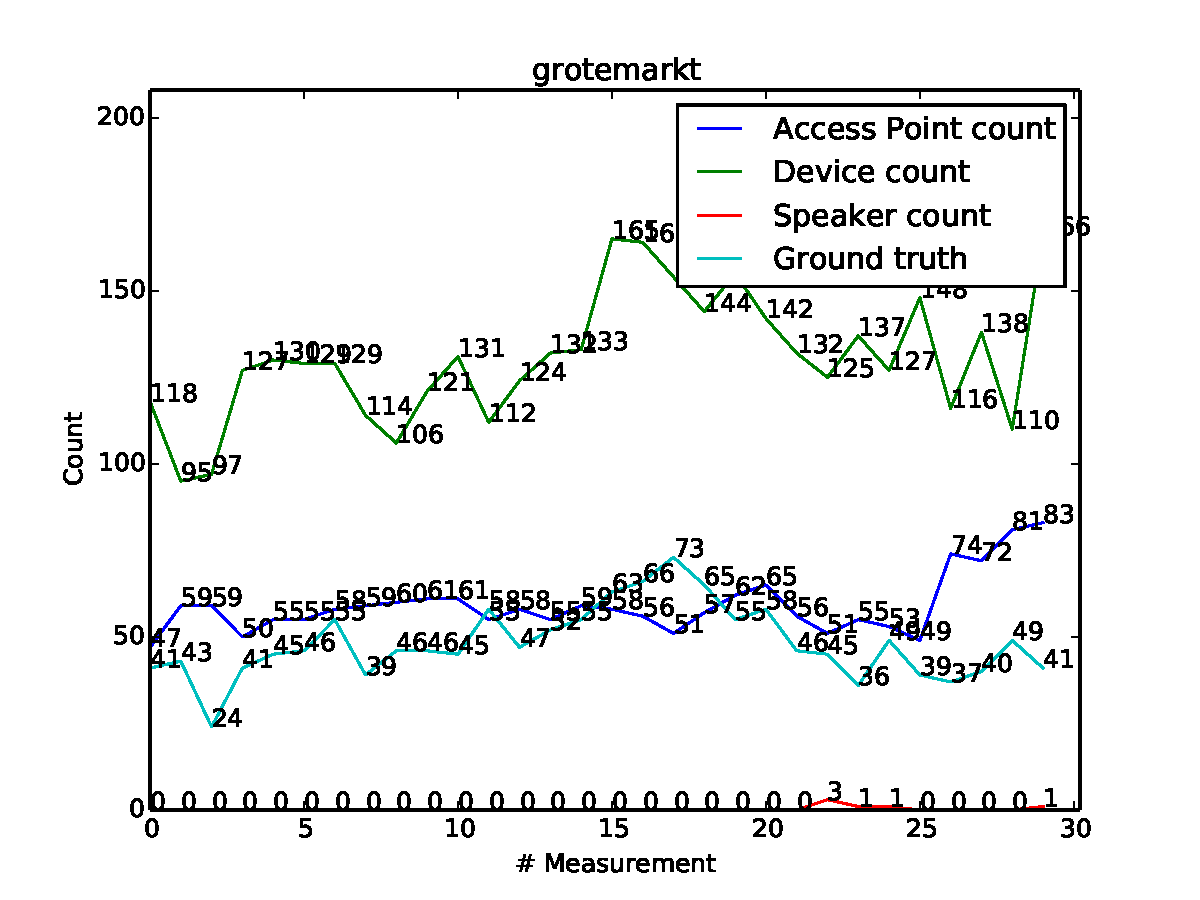
\includegraphics[width=0.7\textwidth]{./img/result/day/day2/grotemarkt-20161027}
    }
  }\\
  \subfloat[day 3]{
    \label{fig:grotemarkt-day3}{
      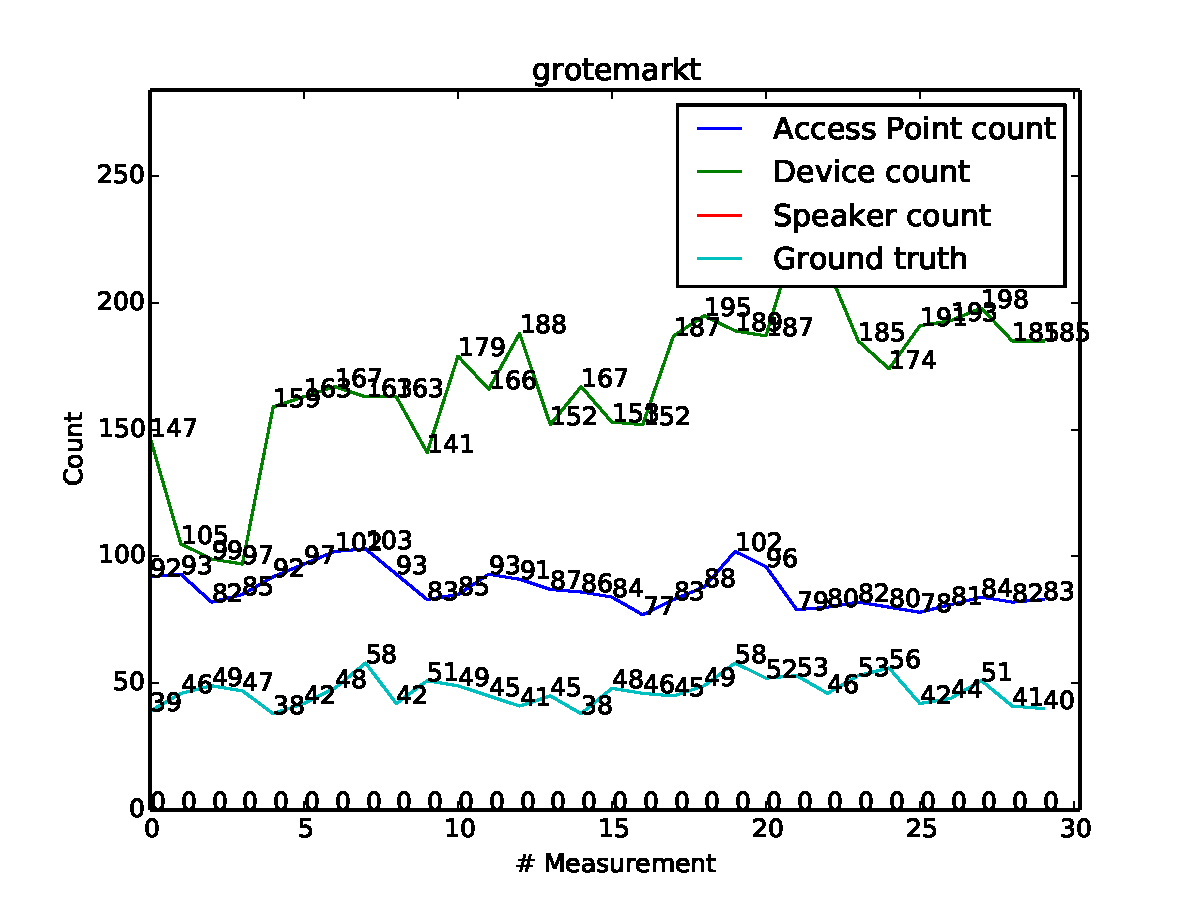
\includegraphics[width=0.7\textwidth]{./img/result/day/day3/grotemarkt-20161028}
    }
  }
  \subfloat[day 4]{
    \label{fig:grotemarkt-day4}{
      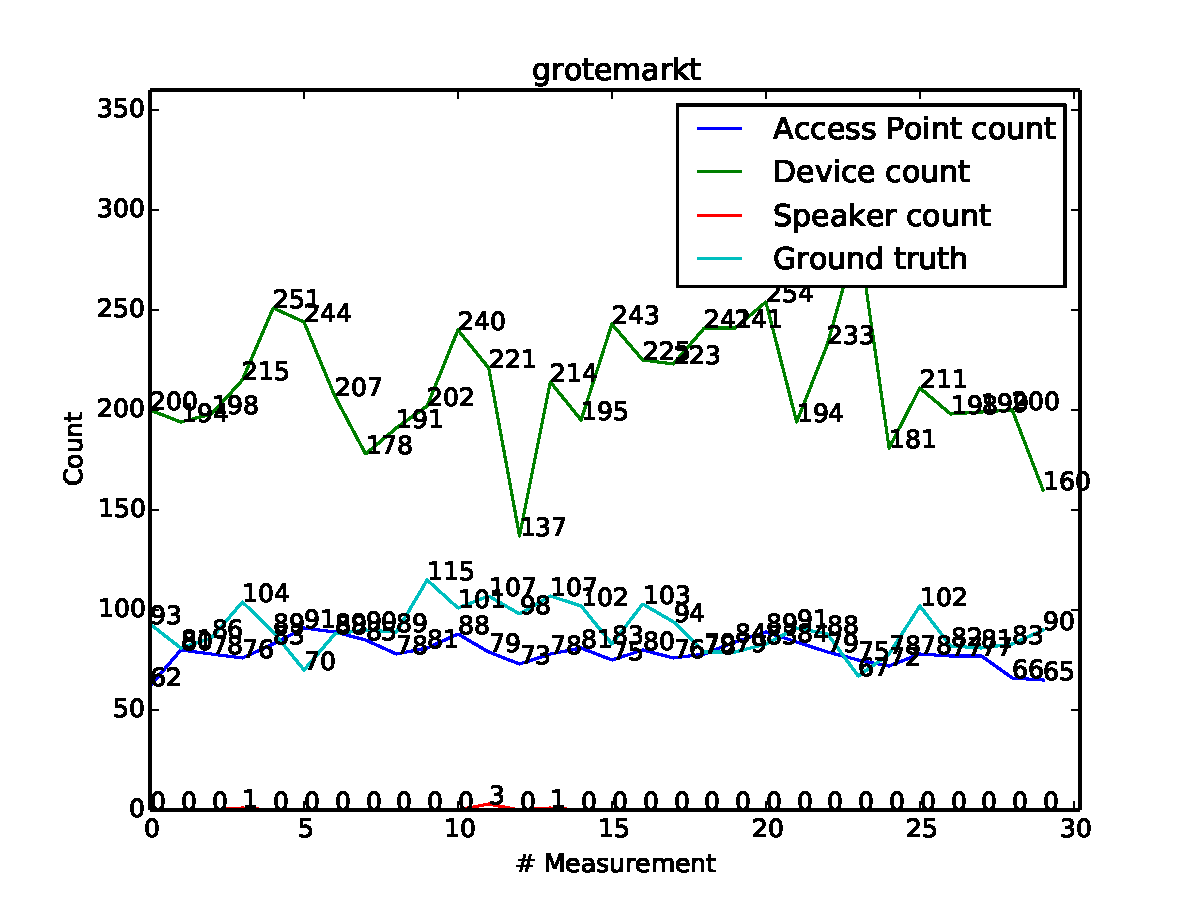
\includegraphics[width=0.7\textwidth]{./img/result/day/day4/grotemarkt-20161029}
    }
  }
  \end{adjustwidth}
  \caption[The line chart of sensor readings at Grote Markt.]
  {The line chart of sensor readings at \textit{Grote Markt} in four days of experiment.}
  \label{fig:result-grotemarkt-line-chart}
\end{figure}


%********************************************************************
% Other Stuff in the Back
%*******************************************************
\cleardoublepage%********************************************************************
% Bibliography
%*******************************************************
% work-around to have small caps also here in the headline
\manualmark
\markboth{\spacedlowsmallcaps{\bibname}}{\spacedlowsmallcaps{\bibname}} % work-around to have small caps also
%\phantomsection 
\refstepcounter{dummy}
\addtocontents{toc}{\protect\vspace{\beforebibskip}} % to have the bib a bit from the rest in the toc
\addcontentsline{toc}{chapter}{\tocEntry{\bibname}}
\label{app:bibliography}
\printbibliography

\cleardoublepage%*******************************************************
% Declaration
%*******************************************************
\refstepcounter{dummy}
\pdfbookmark[0]{Declaration}{declaration}
\chapter*{Declaration}
\thispagestyle{empty}
Put your declaration here.
\bigskip
 
\noindent\textit{\myLocation, \myTime}

\smallskip

\begin{flushright}
    \begin{tabular}{m{5cm}}
        \\ \hline
        \centering\myName \\
    \end{tabular}
\end{flushright}

\cleardoublepage\pagestyle{empty}

\hfill

\vfill


\pdfbookmark[0]{Colophon}{colophon}
\section*{Colophon}
This document was typeset using the typographical look-and-feel \texttt{classicthesis} developed by Andr\'e Miede. 
The style was inspired by Robert Bringhurst's seminal book on typography ``\emph{The Elements of Typographic Style}''. 
\texttt{classicthesis} is available for both \LaTeX\ and \mLyX: 
\begin{center}
\url{https://bitbucket.org/amiede/classicthesis/}
\end{center}
Happy users of \texttt{classicthesis} usually send a real postcard to the author, a collection of postcards received so far is featured here: 
\begin{center}
\url{http://postcards.miede.de/}
\end{center}
 
\bigskip

\noindent\finalVersionString

%Hermann Zapf's \emph{Palatino} and \emph{Euler} type faces (Type~1 PostScript fonts \emph{URW
%Palladio L} and \emph{FPL}) are used. The ``typewriter'' text is typeset in \emph{Bera Mono}, 
%originally developed by Bitstream, Inc. as ``Bitstream Vera''. (Type~1 PostScript fonts were made 
%available by Malte Rosenau and
%Ulrich Dirr.)

%\paragraph{note:} The custom size of the textblock was calculated
%using the directions given by Mr. Bringhurst (pages 26--29 and
%175/176). 10~pt Palatino needs  133.21~pt for the string
%``abcdefghijklmnopqrstuvwxyz''. This yields a good line length between
%24--26~pc (288--312~pt). Using a ``\emph{double square textblock}''
%with a 1:2 ratio this results in a textblock of 312:624~pt (which
%includes the headline in this design). A good alternative would be the
%``\emph{golden section textblock}'' with a ratio of 1:1.62, here
%312:505.44~pt. For comparison, \texttt{DIV9} of the \texttt{typearea}
%package results in a line length of 389~pt (32.4~pc), which is by far
%too long. However, this information will only be of interest for
%hardcore pseudo-typographers like me.%
%
%To make your own calculations, use the following commands and look up
%the corresponding lengths in the book:
%\begin{verbatim}
%    \settowidth{\abcd}{abcdefghijklmnopqrstuvwxyz}
%    \the\abcd\ % prints the value of the length
%\end{verbatim}
%Please see the file \texttt{classicthesis.sty} for some precalculated 
%values for Palatino and Minion.
%
%    \settowidth{\abcd}{abcdefghijklmnopqrstuvwxyz}
%    \the\abcd\ % prints the value of the length





% ********************************************************************
% Game Over: Restore, Restart, or Quit?
%*******************************************************
\end{document}
% ********************************************************************
